\documentclass{article}
\usepackage[]{url}
\usepackage{graphicx}
\usepackage{hyperref}
\usepackage{mathtools}
\usepackage{tikz}
\usepackage{subcaption}
\usepackage{float}
\usepackage{trimclip}

\begin{document}
\title{Collective motion of squirmers in confined environments}
\author{Roth Robin\\
\\
Supervisors: Van Landeghem Céline, Giraldi Laetitia,\\ Agathe Chouippe}
\date{May, 2024}
\maketitle

\tableofcontents
\newpage
\section{Introduction}
This internship is the continuation of a project realised last semester. The main goal of the project was
to develop numerical methods for modeling the dynamics of interacting squirmers. The squirmer is an active particle imitating the propulsion of bacteria.\\
A python code to simulate the behaviors of two interacting squirmers has been implemented during the project.\\
These interactions are governed by steric and lubrification forces.

\section{Context}
The collective behavior of active particles is well studied in the literature. 
The Squirmer model is frequently used to model these active particles. \\
The squirmer model, initially proposed by Lighthill in 1952, represents a spherical Stokesian swimmer with a surface that undergoes small-amplitude deformations to achieve propulsion. This model was enhanced by Blake, who adapted it to describe a spherical microswimmer covered with a dense array of beating cilia. Instead of representing individual cilia, the squirmer model simplifies this by using a continuous, deformable layer that propagates the wave.
This model has been applied to a range of microswimmer dynamics in both biological and artificial contexts..\\
The aim of this internship is to perform a study considering squirmers, 
in various confined domains and to compare the collective motion of the squirmers with that of the active particles using the Squirmer model. 
The motion of the squirmers is simulated using a continuous model that approximates lubrification and 
steric forces\cite{Brumley}\cite{Lauga}.

\section{Objectives}
The main goal is to model the dynamics of a group of squirmers within confined environments and to
 study the influence of numerical parameters on their collective behavior such as alignment.\\
 To achieve this objective, the following tasks will be undertaken:
 \begin{itemize}
     \item To validate the formulas of the steric and lubrification forces from the previous project,
     \item To investigate the impact of altering the parameter $\beta$, which defines the
    type of squirmers (pusher, puller, neutral swimmer), on the interaction between two squirmers,
     \item To conduct a comparative analysis of the interaction between a squirmer and a 
    boundary of the domain by varying the initial angle of the squirmer and the parameter $\beta$, 
    to comprehensively understand their influence on the system dynamics,
     \item To update and optimize the code to enable a simulation of a larger number of squirmers,
     \item To examine the impact of numerical parameters on the collective behavior of squirmers.
\end{itemize}

 

\section{Vicsek model}
\begin{center}
    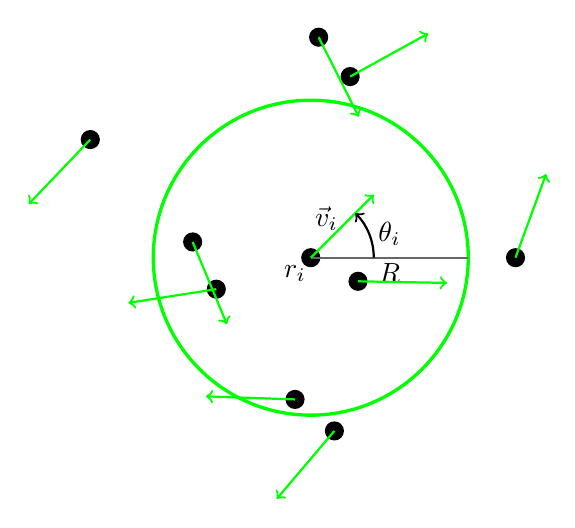
\begin{tikzpicture}
        \draw[color=green, very thick](0,0) circle (2);
        \node at (-0.2,-0.2) {{$r_i$}};
        \filldraw[color=black, fill=black, very thick](0,0) circle(0.1);
        \filldraw[color=black, fill=black, very thick](-1.5,0.2) circle(0.1);
        \filldraw[color=black, fill=black, very thick](0.5,2.3) circle(0.1);
        \filldraw[color=black, fill=black, very thick](2.6,0) circle(0.1);
        \filldraw[color=black, fill=black, very thick](-0.2,-1.8) circle(0.1);
        \filldraw[color=black, fill=black, very thick](0.6,-0.3) circle(0.1);
        \filldraw[color=black, fill=black, very thick](-1.2,-0.4) circle(0.1);
        \filldraw[color=black, fill=black, very thick](-2.8,1.5) circle(0.1);
        \filldraw[color=black, fill=black, very thick](0.3,-2.2) circle(0.1);
        \filldraw[color=black, fill=black, very thick](0.1,2.8) circle(0.1);
        \draw[thick, -, color=black!60] (0,0) -- (2,0);
        \node at (1,-0.2) {{$R$}};
        %Length of the arrow
        \pgfmathsetmacro{\len}{sqrt(1.28)}

        %Draw arrows with random directions
        \foreach \x/\y in {-1.5/0.2, 0.5/2.3, 2.6/0, -0.2/-1.8, -1.2/-0.4, -2.8/1.5, 0.3/-2.2, 0.1/2.8} {
            \pgfmathsetmacro{\angle}{random()*360}
            \draw[thick, ->, color=green] (\x,\y) -- ++({\len*cos(\angle)},{\len*sin(\angle)});
        }
        \draw[thick, ->, color=green] (0,0) -- (0.8,0.8);
        \draw[thick, ->, color=green] (0.6, -0.3) -- ++ ({\len*cos(-1.04)},{\len*sin(-1.04)});
        \node [color=black] at (0.2,0.5) {{$\vec{v}_i$}};
        \draw[thick, ->, color=black] (0.8, 0) arc (0:45:0.8);
        \node at (1, 0.3) {{$\theta_i$}};
    \end{tikzpicture}
\end{center}

The Vicsek model consists of $N$ particles with $r_i(t)$ and $\theta_i(t)$ 
their mass center and orientations.\\
All particles have the same velocity $v_0$ and radius.
The evolution of the orientation $\theta_i(t)$ at each time step $\Delta t$ is:
$$\theta_i(t + \Delta t) = \langle\theta_j(t)\rangle_{|r_i(t) - r_j(t)| < R} + \epsilon_i(t),$$
with
$$\langle\theta_j(t)\rangle = \arctan\left(\frac{\sin(\theta_j(t))}{\cos(\theta_j(t))}\right).$$
$R$ is the range of interaction, $\langle\theta_j(t)\rangle_{|r_i(t) - r_j(t)| < R}$ the average 
orientation of the particles in the range $R$ of
 the $i$-th particle (including itself) at the time $t$ and $\epsilon_i(t)$ represents the noise. 
 It is a random number taken from a uniform probability distribution
over $\left(-\frac{\eta}{2}, \frac{\eta}{2}\right)$ where $\eta$ is the main tool that counteracts the alignment of the particles.\\
\\
The evolution of the position $r_i(t)$ at each time step $\Delta t$ is:
$$ r_i(t + \nabla t) = r_i(t) + v_0\Delta t \begin{pmatrix}
    \cos(\theta_i(t))\\
    \sin(\theta_i(t))
\end{pmatrix}.$$
The velocity $\vec{v}_i(t)$ is defined by:
$$\vec{v}_i(t) = v_0\begin{pmatrix}
    \cos\theta_i(t)\\
    \sin\theta_i(t)
\end{pmatrix}.$$
The behavior of the particles are quantified by the polar order parameter $v_a$ which is given by:
$$v_a = \frac{1}{Nv_0}\left|\sum^{N}_{i=1}\vec{v}_i\right|$$.
The boundary conditions are reflective, if a particle is outside of the domain after computing $r_i(t + \Delta t)$, the new coordinates and orientations are given by:\\
For the x-boundary:
$$|x_i(t + \Delta t)| = 2L_x - |x_i(t + \Delta t)|,$$
$$\theta_{i}(t + \Delta t) = \pi - \theta_i(t + \Delta t).$$
For the y-boundary:
$$|y_i(t + \Delta t)| = 2L_y - |y_i(t + \Delta t)|,$$
$$\theta_i(t + \Delta t) = -\theta_i(t + \Delta t).$$
These conditions ensures that the particles reflect off the boundaries.

\newpage
\section{Squirmer model}
\begin{center}
   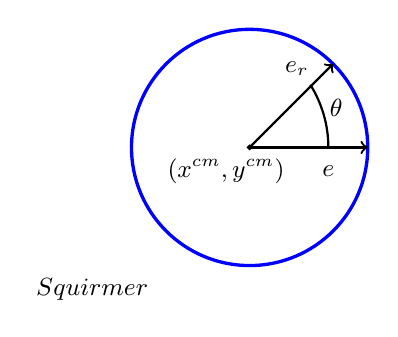
\begin{tikzpicture}
      \small
      
      \draw[color=blue, very thick](2.5,2.5) circle (1.5);
      
      \draw[color=black, very thick](2.5,2.5) circle (0.01);
      
      \node  at (2.5-0.3,2.5-0.3) {{$(x^{cm},y^{cm})$}};
      
      \node  at (0.5,0.7) {{$Squirmer$}};
      
      \draw[thick, ->] (2.5,2.5) -- (4,2.5);
      \node  at (3.5,2.2) {{$e$}};
   
      \pgfmathsetmacro{\xcoord}{2.5 + 1.5*cos(45)}
       \pgfmathsetmacro{\ycoord}{2.5 + 1.5*sin(45)}
       \draw[thick, ->] (2.5,2.5) -- (\xcoord,\ycoord);
      \node  at (3.1,3.5) {{$e_r$}}; 
      \draw[thick, -] (3.5,2.5) arc[start angle=0, end angle=32, radius=1.5];
      \node at (3.6,3) {${\theta}$}; 
      
         
      \end{tikzpicture}
    \end{center}
The time-independent velocity $u$ defined on the surface of the squirmer is given 
in polar coordinates by :

\begin{align*}
   \left\{\begin{array}{rcl}
      u_r(R,\theta) &=& 0 \\
      u_\theta(R,\theta) &=& B_1\mathrm{sin}(\theta)+B_2\mathrm{sin}(\theta)\mathrm{cos}(\theta)
   \end{array}\right.\ \cite{Lauga};
\end{align*}

By setting $\beta=\frac{B_2}{B_1}$, we have :
$$
u_\theta(R,\theta) = B_1(\mathrm{sin}(\theta) + \beta \mathrm{sin}(\theta)\mathrm{cos}(\theta)),
$$
where $\beta$ is the type of the squirmer :
$$\left\{
    \begin{array}{ll}
        \beta = 0 : \text{neutral swimmer}  \\
        \beta < 0 : \mathrm{pusher} \\
        \beta > 0 : \mathrm{puller} \\
    \end{array}
\right.$$
and $B_1$ describes the swimming velocity $v_0 = \frac{2 B_1}{3}$.
\\ Now let us put $u$ in cartesian coordinates :
\begin{align*}
    u &= \begin{pmatrix}
   u_x \\
   u_y
\end{pmatrix}
= \begin{pmatrix}
   \mathrm{cos}(\theta) & -\mathrm{sin}(\theta) \\
   \mathrm{sin}(\theta) & \mathrm{cos}(\theta)
\end{pmatrix}
\begin{pmatrix}
   u_r \\
   u_\theta
\end{pmatrix}, \\
&= B_1 (1 + \beta \mathrm{cos}(\theta))
\begin{pmatrix}
   -\mathrm{sin}^2(\theta) \\
   \mathrm{sin}(\theta)\mathrm{cos}(\theta)
\end{pmatrix}.
\end{align*}

We define $e_r$ the unit vector pointing from the center to the surface 
$$
e_r = \begin{pmatrix}
   \frac{x - x^{cm}}{r}  \\
   \frac{y - y^{cm}}{r} 
\end{pmatrix} = \begin{pmatrix}
   \mathrm{cos}(\theta) \\
   \mathrm{sin}(\theta)
\end{pmatrix}$$ 

and $e$ = 
$\begin{pmatrix}
   \mathrm{cos}(\theta) \\
   \mathrm{sin}(\theta) \end{pmatrix}$ the swimming direction of the squirmer. 
   
   By fixing $\theta$ = 0, one has $e$ = $\begin{pmatrix}
   1 \\
   0 \end{pmatrix}$ and one finds the following expression for the velocity field 
   in cartesian coordinates: 

\begin{align*}
u &= B_1 \left(1+\beta \mathrm{cos}(\theta) \right) \begin{pmatrix}
   -\mathrm{sin}^2(\theta) \\
   \mathrm{sin}(\theta)\mathrm{cos}(\theta)
\end{pmatrix},  \\
&= B_1 \left(1+\beta \mathrm{cos}(\theta) \right) \begin{pmatrix}
   \mathrm{cos}^2(\theta)-1 \\
   \mathrm{sin}(\theta)\mathrm{cos}(\theta)
\end{pmatrix}, \\
&= B_1 \left(1+\beta \begin{pmatrix}
   1 \\
   0 \end{pmatrix}\begin{pmatrix}
   \mathrm{cos}(\theta) \\
   \mathrm{sin}(\theta)
\end{pmatrix}\right) \left[ \left( \begin{pmatrix}
   1 \\
   0 \end{pmatrix}\begin{pmatrix}
   \mathrm{cos}(\theta) \\
   \mathrm{sin}(\theta)
\end{pmatrix}\right) \begin{pmatrix}
   \mathrm{cos}(\theta) \\
   \mathrm{sin}(\theta)
\end{pmatrix} - \begin{pmatrix}
   1 \\
   0 \end{pmatrix}\right], \\
&= B_1(1+\beta (e \cdot e_r)) [(e \cdot e_r)e_r - e]. 
\end{align*}

\vspace{0.5 cm}
Thus, $u$ in cartesian coordinates is given by :
\begin{equation*}
\boxed{u_r = B_1(1+\beta (e\cdot e_r)) [(e\cdot e_r)e_r - e].}
\end{equation*}


\section{Dynamics of two interacting squirmers}
\subsection{The evolution of the mass center $R_i$}
The evolution of the mass center $R_i$ = $(X_i, Y_i)$ of one squirmer $i$ in presence of 
another squirmer $j$ and rigid boundaries, is given by :
\begin{center}
$\boxed{\frac{dR_i}{dt}$ = $v_0 p_i -  \sum\limits_{i \ne j}\nabla_{R_{ij}} V_{ij} - \sum\limits_{i}\nabla_{R_i} V_i + \sum\limits_{i\ne j}\left[F_{i(j)\rightarrow i} + F_{j(i)\rightarrow i}\right]+ \sum\limits_{k \in w}F_{k\rightarrow i}^w + \sqrt{2D}\eta_i(t)}$
\end{center}
We have : \begin{itemize}
    \item $v_0$ the particle swimming velocity,
    \item $p_i$ = $(\mathrm{cos}(\theta),\mathrm{sin}(\theta))$ orientation,
    \item $F_{i(j)\rightarrow k}$ the lubrification forces felt by the $k^{th}$ squirmer and generated by the $i^{th}$ squirmer in presence of the $j^{th}$ one \cite{Brumley},
    \item $F^w_{k\rightarrow i}$ the lubrification forces felt by the $i^{th}$ squirmer and generated by the $k^{th}$ wall\cite{Brumley},
    \item $V_{ij}$ and $V_i$, Weeks-Chandler-Andersen potential : repulsive steric force avoiding the overlapping of two squirmers or of one squirmer and a rigid boundary. The force is activated when the distance between two surfaces is small,
    \item $D$ the translational diffusivity
    \item $\eta_i$'s are independent noises. 
\end{itemize} 
\vspace{0,5cm}
By the second law of Newton, the acceleration is given by:
$$m\vec{a} = \sum\limits_i \vec{F}_i.\cite{Newton}$$
The force of viscosity on a small sphere moving through a viscous fluid is given by the Stokes-Einstein relation:
$$F_d = 6\mu\pi r.\cite{Stokes}$$
The squirmers have no inertia, so $\vec{a} = 0$, such as:
$$0 = -F_d\frac{dR_i}{dt} + \sum\limits_{i \ne d} F_i,$$
we have:
$$\frac{dR_i}{dt} = \frac{1}{6\mu\pi r}\sum\limits_{i \ne d} F_i.$$
The Weeks-Chandler-Andersen potential is then given by:
$V_{ij}$ = $\frac{E_s}{6\pi\mu r}\left[\left(\frac{2r}{\lvert R_{ij}\rvert}\right)^{12} - \left(\frac{2r}{\lvert R_{ij}\rvert}\right)^6\right]$ and  $V_i$ = $\frac{E_s}{6\pi\mu r} \left[ \left( \frac{r}{\lvert R - R_i \rvert} \right)^{12} - \left( \frac{r}{\lvert R - R_i \rvert} \right) ^6 \right]$ 
\vspace{0,3cm}
\\With : \begin{itemize}
    \item $R_{ij}$ = $\sqrt{D_x^2+D_y^2}$, $\lvert R_{ij} \rvert$ the distance between the centers of two squirmers,
    \item $\lvert R - R_i\rvert$ the distance between the wall and the squirmer center,
    \item $E_s$ a positive constant,
    \item $r$ the radius of a squirmer,
    \item $\mu$ the dynamic viscosity.
\end{itemize}

\vspace{0,5cm}
We want to compute the steric force, given by $\nabla_{R_{ij}} V_{ij}$:

\begin{align*}
\frac{\partial V_{ij}}{\partial D_x} &= \frac{\partial}{\partial D_x}\frac{E_s}{6\pi\mu r}\left[\left(\frac{2r}{\lvert R_{ij}\rvert}\right)^{12} - \left(\frac{2r}{\lvert R_{ij}\rvert}\right)^6\right] \\
&= \frac{E_s}{6\pi\mu r} \left[\frac{\partial}{\partial D_x}\left(\frac{2r}{\lvert R_{ij}\rvert}\right)^{12} - \frac{\partial}{\partial D_x} \left(\frac{2r}{\lvert R_{ij}\rvert}\right)^6\right] \\
&= \frac{E_s}{6\pi\mu r} \left[ \frac{-12 D_x (2r)^{12}(R_{ij})^{10}}{(R_{ij})^{24}} - \frac{-6D_x(2r)^6(R_{ij})^4}{(R_{ij})^{12}}  \right] \\
&= \frac{-12 E_s}{2r6\pi\mu r} \left[ \frac{D_x (2r)^{13}}{(R_{ij})^{14}} - \frac{D_x (2r)^{7}}{2(R_{ij})^8}\right] \\
&= -\frac{E_s}{2r^2\pi\mu} \frac{D_x}{R_{ij}} \left[ \frac{2(2r)^{13}}{(R_{ij})^{13}} - \frac{(2r)^7}{(R_{ij})^{7}}\right]
\end{align*}
Equivalently, we have : 
$\frac{\partial V_{ij}}{\partial D_y}$ = $-\frac{E_s}{2r^2\pi\mu} \frac{D_y}{R_{ij}}\left[ \frac{2(2r)^{13}}{(R_{ij})^{13}} - \frac{(2r)^7}{(R_{ij})^7} \right]$
\\ We find : 
\begin{equation*}
    \boxed{\nabla_{R_{ij}} V_{ij} = 
    \begin{pmatrix}
        -\frac{E_s}{2r^2\pi\mu} \frac{D_x}{R_{ij}}\left[ \frac{2(2r)^{13}}{(R_{ij})^{13}} - \frac{(2r)^7}{(R_{ij})^7} \right] \\
        -\frac{E_s}{2r^2\pi\mu} \frac{D_y}{R_{ij}}\left[ \frac{2(2r)^{13}}{(R_{ij})^{13}} - \frac{(2r)^7}{(R_{ij})^7} \right]
    \end{pmatrix}}
\end{equation*}

\vspace{0,5cm}

In addition, we need to compute $\partial_{R_i} V_i$ to obtain the force applied between a squirmer and a rigid boundary.

\begin{align*}
    \frac{\partial V_i}{\partial X} &= \frac{\partial}{\partial X} \left( \frac{E_s}{6\pi\mu r} \left[ \left( \frac{r}{\lvert R - R_i \rvert} \right)^{12} - \left( \frac{r}{\lvert R - R_i \rvert} \right) ^6 \right] \right) \\
    &= \frac{\partial}{\partial X} \left( \frac{E_s}{6\pi\mu r} \left[ \left( \frac{r}{\sqrt{( X_{box}-X)^2 + (Y_{box}-Y)^2}} \right)^{12} - \left( \frac{r}{\sqrt{( X_{box}-X)^2 + (Y_{box}-Y)^2}} \right) ^6 \right] \right) \\
    &= \frac{E_s}{6\pi\mu r}\left[ 12(X_{box}-X)\frac{r^{12}}{\lvert R - R_i\rvert^{14}} - 6(X_{box}-X)\frac{r^6}{\lvert R-R_i\rvert^8} \right] \\
    &= -\frac{E_s (X_{box}-X)}{\pi\mu r^2 \lvert R - R_i \rvert } \left[ 2 \left( \frac{r}{\lvert R-R_i\rvert} \right)^{13} - \left( \frac{r}{\lvert R-R_i\rvert}\right)^7 \right] 
\end{align*}
Equivalently, we have : $\frac{\partial V_i}{\partial Y}$ = $ - \frac{E_s (Y_{box}-Y)}{\pi\mu r^2 \lvert R - R_i \rvert } \left[ 2 \left( \frac{r}{\lvert R-R_i\rvert} \right)^{13} - \left( \frac{r}{\lvert R-R_i\rvert}\right)^7 \right]$

We have : 
\begin{equation*}
    \boxed{\nabla_{R_i} V_i = \begin{pmatrix}
        - \frac{E_s (X_{box}-X)}{\pi\mu r^2 \lvert R - R_i \rvert } \left[ 2 \left( \frac{r}{\lvert R-R_i\rvert} \right)^{13} - \left( \frac{r}{\lvert R-R_i\rvert}\right)^7 \right] \\
        - \frac{E_s (Y_{box}-Y)}{\pi\mu r^2 \lvert R - R_i \rvert } \left[ 2 \left( \frac{r}{\lvert R-R_i\rvert} \right)^{13} - \left( \frac{r}{\lvert R-R_i\rvert}\right)^7 \right]
    \end{pmatrix}}
\end{equation*}

\begin{center}
   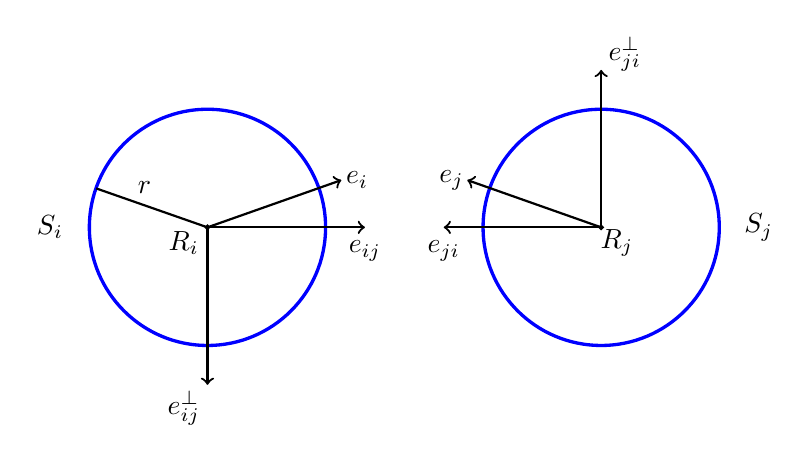
\begin{tikzpicture}
   
   \draw[color=blue, very thick](5,5) circle (1.5);
   \draw[color=blue, very thick](0,5) circle (1.5);
   
   \draw[color=black, very thick](0,5) circle (0.01);
   \draw[color=black, very thick](5,5) circle (0.01);
   
   \node  at (-0.3,5-0.2) {{$R_i$}};
   \node  at (5+0.2,5-0.2) {{$R_j$}};
   
   \node  at (-2,5) {{$S_i$}};
   \node  at (7,5) {{$S_j$}};
   
   \draw[thick, ->] (0,5) -- (1.7,5+0.6);
   \draw[thick, ->] (5,5) -- (5-1.7,5+0.6);
   
   \node  at (1.9,5+0.6) {{$e_i$}};
   \node  at (5-1.9,5+0.6) {{$e_j$}};
   
   \draw[thick] (0,5) -- ({-cos(45)*2}, {5+0.7*sin(45)});
   \node  at (-0.8,5+0.5) {{$r$}};
   
   \draw[thick, ->] (0,5) -- (2,5);
   \draw[thick, ->] (5,5) -- (3,5);
   
   \node  at (2,5-0.3) {{$e_{ij}$}};
   \node  at (3,5-0.3) {{$e_{ji}$}};
   
   \draw[thick, ->] (0,5) -- (0,3);
   \node  at (-0.3,3-0.3) {$e^{\perp}_{ij}$};
   
   
   \draw[thick, ->] (5,5) -- (5,7);
   \node  at (5+0.3,7+0.2) {$e^{\perp}_{ji}$};
   
   \end{tikzpicture}
   \end{center}
The figure shows the different vectors involved in the computations which will follow.
\\We define : 
\begin{itemize}
    \item $W_n(\mathrm{cos}(\theta))$ = $\frac{2}{n(n+1)}P_n'(\mathrm{cos}(\theta))$ \cite{Brumley}
    \item $P_n(\mathrm{cos}(\theta))$ the Legendre polynomials \cite{Wikipedia}
    \item $p_i\hat{R}_{ij} = -e_i.e_{ij}$
    \item $p_i\hat{R}^{\perp}_{ij}$ = $-\frac{(Y_{R_j} - Y_{R_i})\mathrm{cos}(\theta) - (X_{R_j} - X_{R_i})\mathrm{sin}(\theta)}{\lvert R_{ij} \rvert} $
\end{itemize}

The tangential lubrification forces acting on the two spheres can be calculated explicitly by:
\\ $F_{i(j)\rightarrow i}^{y}$ = $-9 \mu \pi r \frac{\lambda ^2}{(\lambda +1)^2} \sum_{n} \left[ B_n W_n(p_i\hat{R}_{ij})(-p_i\hat{R}_{ij}) + \frac{1}{2} B_n W_n'(p_i\hat{R}_{ij})(p_i\hat{R}^{\perp}_{ij})^2 \right] (ln \epsilon + O(1)).$ \cite{Brumley}

For $n$ = 1 : \begin{align*}
    W_1(p_i\hat{R}_{ij}) &= 1 \\
    W_1'(p_i\hat{R}_{ij}) &= 0 \\
    -B_1 W_1(p_i\hat{R}_{ij})p_i\hat{R}_{ij} + \frac{1}{2} B_1  W_1'(p_i\hat{R}_{ij}) (p_i\hat{R}^{\perp}_{ij})^2  &= -B_1 p_i\hat{R}_{ij}.
\end{align*} 
For $n$ = 2 : \begin{align*}
    W_2(p_i\hat{R}_{ij}) &= p_i\hat{R}_{ij} \\
    W_2'(p_i\hat{R}_{ij}) &= 1\\
    -B_2 W_2(p_i\hat{R}_{ij})p_i\hat{R}_{ij}+ \frac{1}{2} B_2  W_2'(p_i\hat{R}_{ij}) (p_i\hat{R}^{\perp}_{ij})^2  &= -B_2 (p_i\hat{R}_{ij})^2 + \frac{1}{2} B_2(p_i\hat{R}^{\perp}_{ij})^2.
\end{align*}  

We have $B_1 = \frac{3}{2}v_0$, $B_2 = B_1\cdot\beta$ and $\lambda=1$, so:
\begin{align*}
\footnotesize
6\mu\pi rF_{i(j)\rightarrow i}^{y} = -9 \mu \pi r \frac{\lambda ^2}{(\lambda +1)^2} \left[ -B_1 p_i\hat{R}_{ij} -B_2 (p_i\hat{R}_{ij})^2 + \frac{1}{2} B_2(p_i\hat{R}^{\perp}_{ij})^2\right](ln \epsilon + O(1))\\
= -9 \mu \pi r \frac{1}{4}\cdot\frac{3}{2}v_0\left[ -p_i\hat{R}_{ij} -\beta (p_i\hat{R}_{ij})^2 + \frac{1}{2} \beta(p_i\hat{R}^{\perp}_{ij})^2\right](ln \epsilon + O(1))
\end{align*}
\begin{equation*}
\boxed{
    F_{i(j)\rightarrow i}^{y} = \frac{9}{16}v_0
\left[(p_i\hat{R}_{ij})(1 + \beta p_i\hat{R}_{ij}) - \frac{1}{2}\beta(p_i\hat{R}^{\perp}_{ij})^2\right](ln \epsilon + O(1))
}
\end{equation*}
\normalsize
\vspace{0.5cm}

The normal forces acting on the two spheres can be calculated explicitly by: \\
 $F_{i(j)\rightarrow i}^{x}$ = $-\frac{4}{5} \mu \pi r \frac{\lambda(\lambda +4)}{(\lambda +1)^2} \sum_{n} B_n W_n(p_i\hat{R}_{ij}) (ln \epsilon + O(1))$ \cite{Brumley}
\\ So :
\begin{align*}
    \footnotesize
    6\mu\pi rF_{i(j)\rightarrow i}^{x} = -\frac{4}{5}\mu\pi r\frac{5}{4}p_i\hat{R}^{\perp}_{ij}(B_1 + B_2 p_i\hat{R}_{ij})(ln \epsilon + O(1))\\
    = -\mu\pi r\frac{3}{2}v_0p_i\hat{R}^{\perp}_{ij}(1 + \beta p_i\hat{R}_{ij})(ln \epsilon + O(1))
\end{align*}
\begin{equation*}
    \footnotesize
    \boxed{F_{i(j)\rightarrow i}^{x} = -\frac{1}{4}v_0p_i\hat{R}^{\perp}_{ij}(1 + \beta p_i\hat{R}_{ij})(ln \epsilon + O(1))}
\end{equation*}

The effect of a wall can be calculated by replacing one of the spheres with one of infinite diameter:
\begin{equation*}
    \footnotesize
    \boxed{F_{w\rightarrow i}^{y} = \frac{9}{4} v_0
    \left[(p_i\hat{R}_{ij})(1 + \beta p_i\hat{R}_{ij}) - \frac{1}{2}\beta(p_i\hat{R}^{\perp}_{ij})^2\right](ln \epsilon + O(1))}\\
\end{equation*}
\begin{equation*}
    \footnotesize
    \boxed{F_{w\rightarrow i}^{x} = -\frac{1}{5} v_0p_i\hat{R}^{\perp}_{ij}(1 + \beta p_i\hat{R}_{ij})(ln \epsilon + O(1))}
\end{equation*}

\subsection{The evolution of the orientation}
The evolution of the orientation of one squirmer is given by : 
$$
\boxed{\frac{d \theta_i}{dt} = \sum\limits_{i\ne j} \left[\Gamma_{i(j)\rightarrow i} + \Gamma_{j(i)\rightarrow i}\right] + \sum\limits_{k\in w} \Gamma_{k\rightarrow i}^w + \sqrt{2D_o} \eta_o^{(i)}}.
$$
We have:
\begin{itemize}
    \item $\Gamma_{i(j)\rightarrow k}$ the torque exerted on the $k^{th}$ particle by the flow associated to the $i^{th}$ particle, but perturbed by the presence of the $j^{th}$ particle,
    \item $\Gamma_{k\rightarrow i}^w$ the torque exerted on the $i^{th}$ particle by the interactions with the $k^{th}$ walls,
    \item $D_o$ the angular diffusivity is equal to $\frac{3D}{4r^2}$,
    \item $\eta_o^{(i)}$ the noises, independent of $\eta^{i}$.
\end{itemize}
\vspace{0.5cm}
Similarly as with the forces, we have $\phi = 8\pi\mu r^3$ the rotation flow around a sphere\cite{Stokes}:
$$\frac{d \theta_i}{dt} = \frac{1}{\phi}\sum\limits_{i \ne \phi}F_i\cite{Newton}.$$
The torques acting on the squirmer $i$ can be calculated explicitly by: \\
$\Gamma_{i(j)\rightarrow i}$ = $\frac{16 \lambda}{5(\lambda +1)} \mu \pi r^2 p_i\hat{R}_{ij}^{\perp}\sum_{n} B_n W_n(p_i\hat{R}_{ij}) (ln \epsilon + O(1))$ \cite{Brumley}
\\ So :
\begin{align*}
    \footnotesize
    \phi \Gamma_{i(j)\rightarrow i} = \frac{8}{5}\mu\pi r^2p_i\hat{R}_{ij}^{\perp}(B_1 + B_2 p_i\hat{R}_{ij})(ln \epsilon + O(1))\\
    = \frac{8}{5}\mu\pi r^2p_i\hat{R}_{ij}^{\perp}\frac{3}{2}v_0(1 + \beta p_i\hat{R}_{ij})(ln \epsilon + O(1))
\end{align*}
\begin{equation*}
    \boxed{\Gamma_{i(j)\rightarrow i} = \frac{3}{10}\frac{v_0}{r}p_i\hat{R}_{ij}^{\perp}(1 + \beta p_i\hat{R}_{ij})(ln \epsilon + O(1))}
\end{equation*}

The torques acting on the squirmer $j$ can be calculated explicitly by : \\
$\Gamma_{i(j)\rightarrow j}$ = $\frac{4 \lambda^2}{5(\lambda +1)} \mu \pi r^2 p_i\hat{R}_{ij}^{\perp}\sum_{n} B_n W_n(p_i\hat{R}_{ij}) (ln \epsilon + O(1))$ \cite{Brumley}
\\ So :
\begin{align*}
    \footnotesize
    \phi \Gamma_{i(j)\rightarrow j} = \frac{2}{5}\mu\pi r^2p_i\hat{R}_{ij}^{\perp}(B_1 + B_2 p_i\hat{R}_{ij})(ln \epsilon + O(1))\\
    = \frac{2}{5}\mu\pi r^2p_i\hat{R}_{ij}^{\perp}\frac{3}{2}v_0(1 + \beta p_i\hat{R}_{ij})(ln \epsilon + O(1))
\end{align*}
\begin{equation*}
    \boxed{\Gamma_{i(j)\rightarrow j} = \frac{3}{40}\frac{v_0}{r}p_i\hat{R}_{ij}^{\perp}(1 + \beta p_i\hat{R}_{ij})(ln \epsilon + O(1))}
\end{equation*}
One can note that for two squirmers having the same radius $r$, $\lambda = 1$ and:
$$\Gamma_{i(j)\rightarrow j} = \frac{1}{4}\Gamma_{i(j)\rightarrow i}$$

Similarly as for the forces, the torques produced by the walls can be calculated by replacing one of the spheres with one of infinite diameter:
\begin{equation*}
    \boxed{\Gamma_{w\rightarrow i} = \frac{3}{5} \frac{v_0}{r}p_i\hat{R}_{ij}^{\perp}(1 + \beta p_i\hat{R}_{ij})(ln \epsilon + O(1))}
\end{equation*}



\section{Implementation}
In this section we will detail the files of the \texttt{\href{https://github.com/master-csmi/2024-m1-nemo/tree/main/Code}{Code}} directory,
it is detailed with comments within the code itself.
\subsection{vicsek}
\subsubsection*{Parameters}
\begin{itemize}
    \item $N$ the number of particles in the system
    \item $R$ the range of interaction of the particles
    \item $L$ the length of the square
    \item $v0$ the constant velocity of the particles
    \item $radius$ the radius of the particles
    \item $T$ the time of simulation
    \item $dt$ the time step
    \item $noise$ the $\eta$ parameter, used to counteract the alignment of the particles
\end{itemize}
The class initializes $N$ particles with random position and orientation within the square. The square has reflective boundary conditions.
\subsubsection*{Methods}
\begin{itemize}
    \item \texttt{distance(p1, p2)} returns the distance between \texttt{p1} and \texttt{p2}.
    \item \texttt{dist\_particles(particle)} returns a list which contains the distances between the particle and all other particles of the system.
    \item \texttt{how\_many\_in\_square()} prints and returns the percentage of particles inside the square. It is
    used to test if the code contains errors.
    \item \texttt{ploar\_order\_parameter()} computes and returns $v_a$ the polar order parameter.
    \item \texttt{ref\_border\_x(particle, boundary)} and \texttt{ref\_border\_y(particle, boundary)}
    simulates the reflective borders.
    \item \texttt{vector\_x(p1, p2)} and \texttt{vector\_y(p1, p2)} return respectively the vector in the x and y direction of \texttt{p1} and \texttt{p2}.
    \item \texttt{average\_orient(particle)} returns the average orientation of the particles in a range $R$ of the particle in argument (including itself).
    \item \texttt{update\_orient()} computes the orientation $\theta_i(t + \Delta t)$ using \texttt{average\_orient}.
    \item \texttt{update\_position()} computes the position $r_i(t + \Delta t)$ using the reflective boundaries if necessary
    \item \texttt{loop\_time()} uses \texttt{update\_orientation()} and \texttt{update\_position()} for each time iteration.
    \item \texttt{plot(ax)} plots the square and the particles.
\end{itemize}

\subsection{simulation}
\begin{itemize}
   \item \texttt{sim\_vicsek(N)} used to simulate the behaviors of \texttt{N} particles in a square with the Vicsek model. \texttt{loop\_time} is 
   used and a graph is made with
   the positions and orientations of the particles for each \texttt{step} in \texttt{nb\_step}
\end{itemize}

\subsection{codemat}
This file is the original matlab code that was the base of the study.

\subsection{squirmer}
The first file contains the \texttt{Squirmer} class which takes the initial parameters: 
\begin{itemize}
   \item coordinates \texttt{x} and \texttt{y}
   \item \texttt{orientation}
   \item \texttt{radius}
   \item \texttt{beta}
   \item \texttt{velocity}
\end{itemize}
of a squirmer and computes \texttt{B1} and \texttt{B2}.

\subsection{csv\_file}
This file contains two functions:
\begin{itemize}
   \item \texttt{export\_data\_csv(filename, data)} takes a file name and data from \texttt{loop\_time()} (section \texttt{interactingsquirmers}) and exports it.
   \item \texttt{read\_csv\_file(filename)} takes a file name and returns the data, not currently utilized but may be usefull for future functions.
\end{itemize}

\subsection{plot}
\begin{itemize}
   \item \texttt{plot\_sim\_nsquirmers(histories, Nx, Ny, N, a, border, sim\_border, filename, dir)} takes \texttt{histories}
   the liste returned by \texttt{loop\_time}, \texttt{Nx} and 
   \texttt{Ny} the length and width of the rectangle, \texttt{N} the number of squirmers, \texttt{a} the radius of the squirmers,
   \texttt{border} a boolean which determines if the borders are plotted or not, \texttt{sim\_border} a boolean which is only \texttt{True}
    when a simulation with a single border and a single squirmer is done, \texttt{filename} and \texttt{dir} the names 
    of the file and directory in which the graph is saved.\\
   It then plots the evolution of each squirmer's position over time, a circle is plotted at the initial position, at
   half of the time of the simulation and at the end of the simulation,
   the radius of the circle plotted is proportional to the radius of the squirmers.\\
   This function is used for simulations with a small number of Squirmers and a low simulation time.
   \item \texttt{plot\_time(interact, list\_plot, filename, label, dir)} takes \texttt{interact} an \texttt{Interactingsquirmers}
   , \texttt{list\_plot}, the list to plot over time, usually the list of the minimal distance between the squirmers or the liste of the polar parameter,
   \texttt{label} is a string used for the y-label in the graph and \texttt{filename} and \texttt{dir} is the name of the file
    and directory in which the graph will be saved.\\
    This function is used to plot the minimal distance between squirmers and the polar order parameter over time.
   \item \texttt{create\_video\_from\_history(history, Nx, Ny, N, a, filename, dir, fps)} takes \texttt{history}
   the list of \texttt{loop\_time}, \texttt{Nx} and \texttt{Ny} the length and width of the rectangle,
   \texttt{N} the number of squirmers, \texttt{a} the radius of the squirmers, \texttt{filename} and \texttt{dir}
   the name of the file and directory in which the video is saved, \texttt{fps} the number of frames per second.
    This function is used to create videos with a high number of squirmers and a long simulation time.
\end{itemize}

\subsection{interactingsquirmers}
\subsubsection*{Parameters}
This file implements the \texttt{Interactingsquirmers} class which takes:
\begin{itemize}
   \item \texttt{N}, the number of squirmers
   \item \texttt{xs}, \texttt{ys} and \texttt{orientations} the positions and orientations of the squirmers
   \item \texttt{radius}, the radius of the squirmers
   \item \texttt{beta}, the $\beta$ parameter
   \item \texttt{v0}, the velocity $v_0$
   \item \texttt{Nx} and \texttt{Ny}, the length and width of the rectangle
   \item \texttt{dt}, the time step and \texttt{dt\_out} the time step for output
   \item \texttt{T}, the final time of simulation
   \item \texttt{Es}, the amplitude (intensity) of steric interactions
   \item \texttt{ds}, the distance where the steric interactions become significative
   \item \texttt{mu}, the viscosity
   \item \texttt{R}, the distance which defines if a particle is seen as a neighbour for the clustering order parameter
   \item \texttt{lnEps\_cr}, threshold value for \( -\log(\epsilon) \)
   \item \texttt{D}, the translational diffusivity $D$
   \item \texttt{n} and \texttt{no} the noises associated with the forces and torques
   \item \texttt{border}, a boolean which defines if the simulation is made in a box(\texttt{True}) or a chanel(\texttt{False})
\end{itemize}

\subsubsection*{Methods}
This class has many functions:
\begin{itemize}
   \item \texttt{is\_in\_rectangle()} and \texttt{check\_squirmers\_rectangle()} verify if the squirmers 
    are initially in the rectangle.
   \item \texttt{polar\_order\_parameter()} returns the polar order parameter $v_a$.
   \item \texttt{distance\_all()} returns \texttt{(Dx, Dy, dists)} the directional vector of $R_{i}$ to $R_{j}$ 
   and the distance between each squirmer.
   \item \texttt{forcesSteric(Dxs, Dys, dists)} returns the steric forces \texttt{(Fs\_x, Fs\_y)} computed with the directional vector and the distance calculated with \texttt{distance\_all()}.
   \item \texttt{forcesLubrification(Dx, Dy, dist, theta)} and \texttt{torquesLubrification(Dx, Dy, dist, theta)}
   returns the lubrification forces and torques.
   \item \texttt{compute\_force\_squirmer\_border\_x(self, xs, ys)} and \texttt{compute\_force\_squirmer\_border\_y(self, xs, ys)}
   computes and returns the steric forces between the squirmers and the according walls.
   \item \texttt{force\_torque\_lubrification\_border\_x(self, xs, theta, border)} and \texttt{force\_torque\_lubrification\_border\_y(self, ys, theta, border)}
   computes and returns the lubrification forces and torques between the squirmers and the according walls.
   \item \texttt{ref\_border\_x(self, xs, orientation, boundary)} and \texttt{ref\_border\_y(self, xs, orientation, boundary)} simulates reflective borders when \texttt{border} is \texttt{True}.
   \item \texttt{perio\_border\_x(self, xs, boundary)} simulates periodic borders when \texttt{border} is \texttt{False}.
   \item \texttt{loop\_time()} is the primary function which updates the positions and orientations of each squirmer
   for each time step \texttt{dt} based on the steric forces and the lubrification forces and torques, then updates four list, \texttt{self.vector\_min\_dist} for the minimal 
   distance between the squirmers, \texttt{self.list\_polar} for the polar order parameter, \texttt{self.list\_cluster\_param} for 
   the clustering order parameter and \texttt{history} for the positions, orientations,
   forces and torques at each time step \texttt{dt\_out}. The function then returns \texttt{history}.
   \item \texttt{run(choice, N, a, beta, v0, Nx, Ny, dt, dt\_out, T, Es, ds, mu, R, lnEps\_cr, D, n, no, border, filename, border\_plot)}
   is used to run a simulation, it takes the argument \texttt{choice} that can be:
   \begin{itemize}
    \item 'plot' to plot the graph of the behaviors of the squirmers in the 'graphs' directory, used for a small number of squirmers and a low simulation time,
    \item 'video' to create a video of the behaviors of the squirmers in the 'videos' directory, used for a large number of squirmers or a high simulation time,
    \item 'Eo\_sim', not used anymore, to test the Eo parameter,
    \item 'border', to simulate the behaviors of a squirmer near a wall, only plot possible
    \item 'sim\_2\_sq', to simulate the behaviors of two squirmers near each other, plot and video possible
    \item 'sim\_D', to simulate the influence of the D parameter on the squirmers' behaviors, only video possible.
   \end{itemize}
\end{itemize}

\subsection{Reproducibility-\texttt{run.py}}
The file \texttt{run.py} is utilized to define the parameters and to choose the simulation to make.\\
 To execute the simulations, run the following command:
 \begin{verbatim}
   python Code/run.py sim_choice N filename
\end{verbatim} 
with \texttt{N} the number of squirmers and \texttt{filename} the name of the file in which the resulting graph or video will be stored.
\texttt{sim\_choice} can be:
\begin{itemize}
   \item \texttt{vicsek} to simulate the behaviors of \texttt{N} particles using the Vicsek model.
   \item \texttt{video} to run a simulation with \texttt{N} squirmers and to store the resulting video of the squirmers behaviors and the graphs of the 
   minimum distance between squirmers, the polar order parameter and the clustering order parameter over time
    in the \texttt{videos} directory.
   \item \texttt{plot} to run a simulation with \texttt{N} squirmers and to store the resulting graphs of the squirmers behaviors, the
   minimum distance between squirmers, the polar order parameter and the clustering order parameter over time
    in the \texttt{graphs} directory.
   \item \texttt{Eo\_sim} used at the start of the internship to study the impact of the \texttt{Eo} parameter on the behaviors,
   not used anymore.
   \item \texttt{border} to run twenty simulations between a squirmer and a wall, four simulations is made per \texttt{beta} in the \texttt{betas}
   list in the \texttt{run} function in the \texttt{interactingsquirmers} file. The graphs are stored in the \texttt{graphs/simulations/border/betalabel}
   directory with \texttt{betalabel} the label of \texttt{beta}.
   \item \texttt{sim\_2\_sq} to simulate the behaviors of two squirmers near each other for five $\beta$ values. The
   resulting graphs or videos are stored in the \texttt{graphs/simualtions/sim\_sq\_sq/labelbeta} or the \texttt{videos/simualtions/sim\_sq\_sq/labelbeta}
   directory.
   \item \texttt{sim\_D} to simulate the behaviors of \texttt{N} squirmers for different \texttt{D} values, the resulting graphs
   and videos are stored in the \texttt{videos/simulations/sim\_D} directory.
\end{itemize}

\subsection{Tests}
Two tests are implemented to validate a simulation. The first test is in the \texttt{loop\_time()} of the \texttt{Interactingsquirmers} class.
At each time step, the value of the forces verify:
$$F\cdot dt < v_0,$$
where $F$ represents the steric and lubrification forces.\\
The second test is executed upon a push or a pull request. This test performs a simulation with $375$ squirmers in a box
with reflective borders and test if at any point during the simulation a negative distance has been registered.

\newpage
\section{Numerical Experiments}
\subsection{Simulation of two interacting squirmers}
In this section, forty simulations are conducted involving two closely positioned squirmers. 
The parameters of one squirmer remain fixed throughout all simulations except for its $\beta$ value, while 
the initial orientation and $\beta$ value of the other squirmer are varied. The five $\beta$ values used are:
$$\beta_0 = 0, \beta_1 = 1.5, \beta_2 = 3, \beta_3 = -1.5, \beta_4 = -3.$$ 
The left squirmer is fixed with a radius of $a=0.05$ placed at $(-a, 0)$, a velocity of $v_0=1$ and an initial orientation
of $\theta_1 = \frac{\pi}{2}$ and a $\beta$ value varying among $\beta_0$, $\beta_1$, $\beta_2$, $\beta_3$ and $\beta_4$.\\
The right squirmer, with the same radius $a$ and velocity $v_0$, is placed at $(\frac{2a}{1.9})$. Its orientation $\theta_2$
varies across the principal orientations of the unit circle and its $\beta$ value also varies among $\beta_0$, $\beta_1$, $\beta_2$, $\beta_3$ and $\beta_4$.
We then compare our results to those of a previous study.
\begin{center}
    Behavior observed in a previous study.
    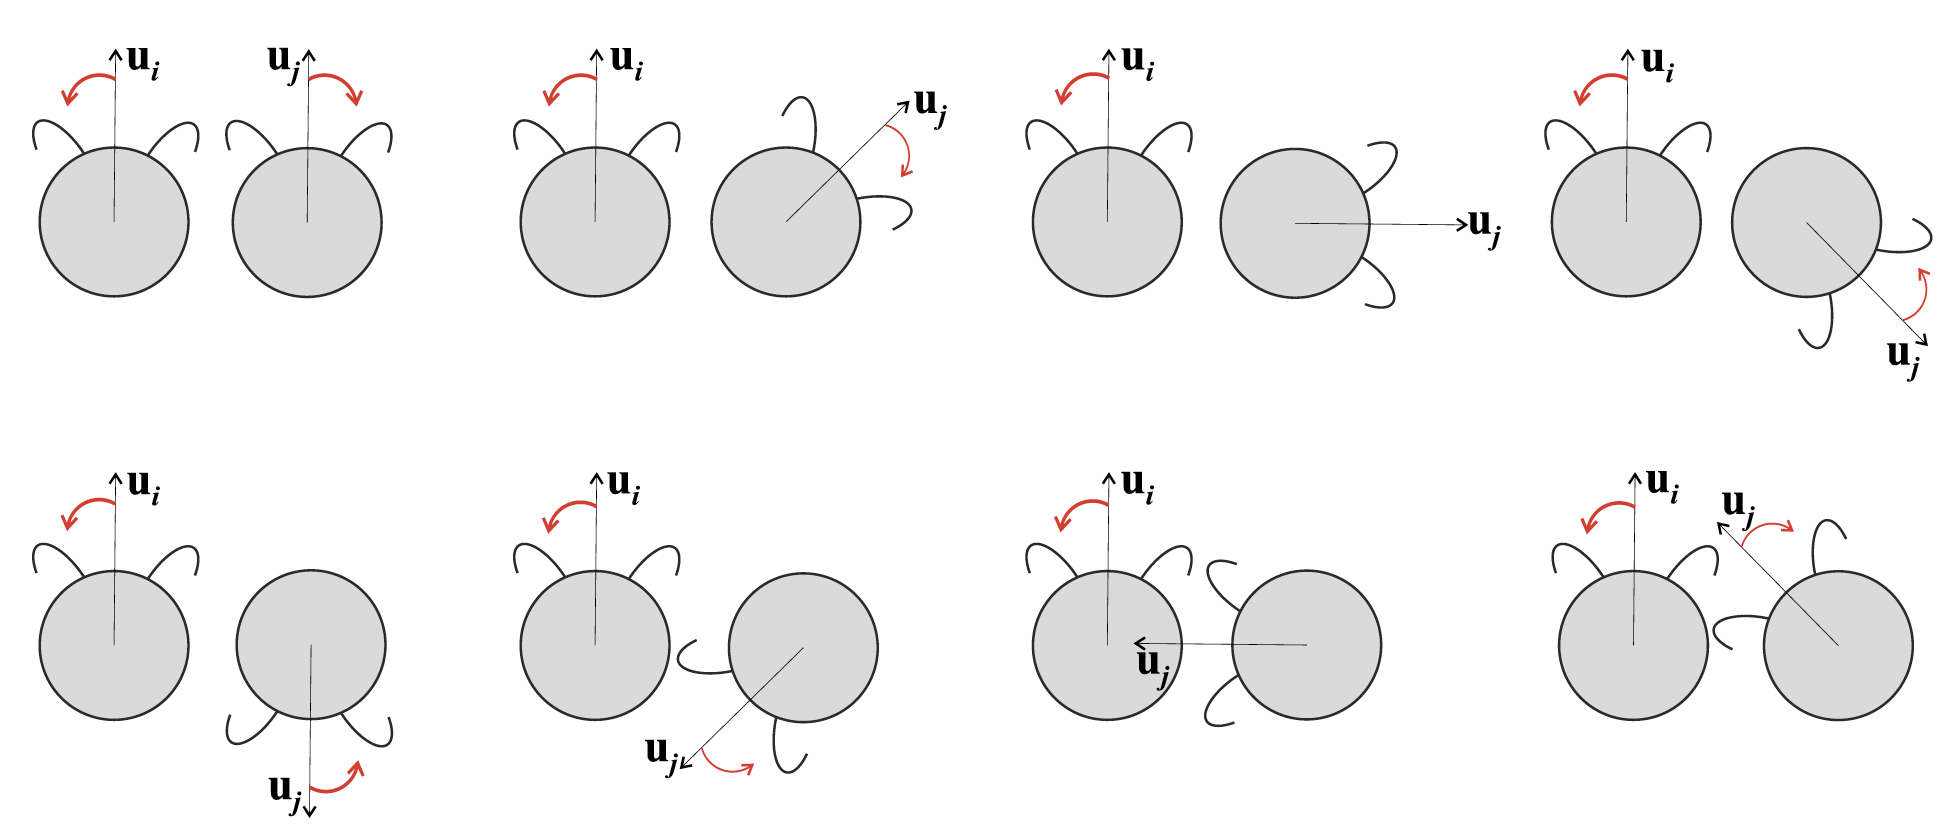
\includegraphics[width=1\textwidth]{Presentation/images/stark_behavior.png}\\
    \cite{Stark}\\
    $u_i$ and $u_j$ the current orientational vector and the rotation due to interaction shown in red.  
 \end{center}
 One can execute these simulations by running the command:
 \begin{verbatim}
    python Code/run.py sim_2_sq 2 filename
 \end{verbatim}
 The parameters can be changed in the \texttt{Code/run.py} and \texttt{Code/interactingsquirmers.py} files.\\
 We show the trajectories of the two squirmers as well as their initial orientation. The grey lines 
 represent the trajectories of the squirmers without any applied forces. Circles are plotted at the start, 
 middle, and end of the simulation, with their radii proportional to the squirmers' sizes.
\newpage
 \begin{figure}[H]
    \centering
    \textbf{$\theta_2 = \frac{\pi}{2}$}\par\medskip
    \begin{minipage}{0.49\textwidth}
        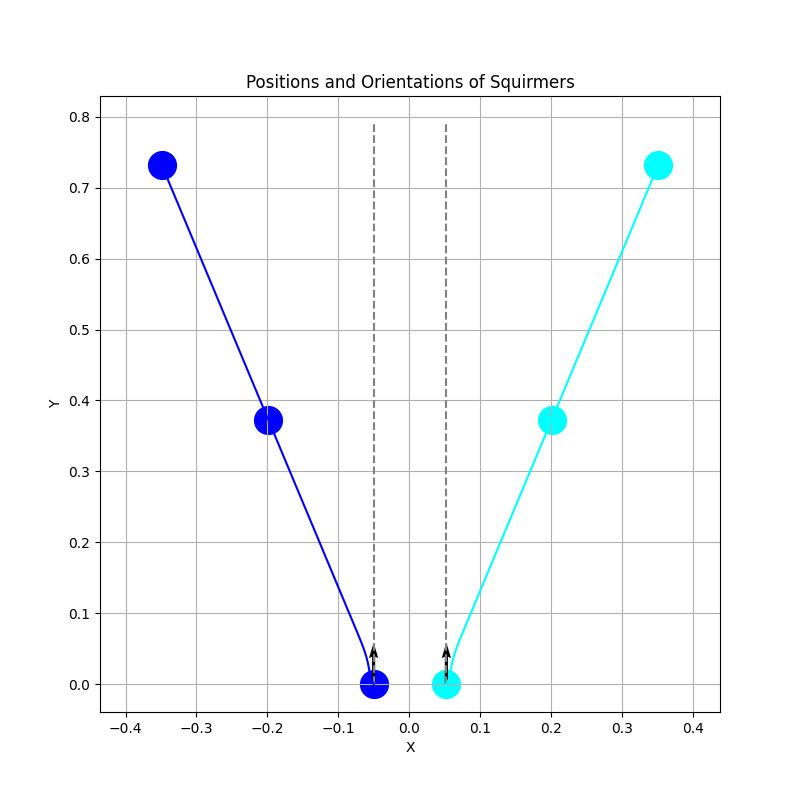
\includegraphics[width=1.1\textwidth]{graphs/simulations/sim_sq_sq/beta3/pi_2_.png}
        \caption{\footnotesize $\beta = 3$}
    \end{minipage}\hfill
    \begin{minipage}{0.49\textwidth}
        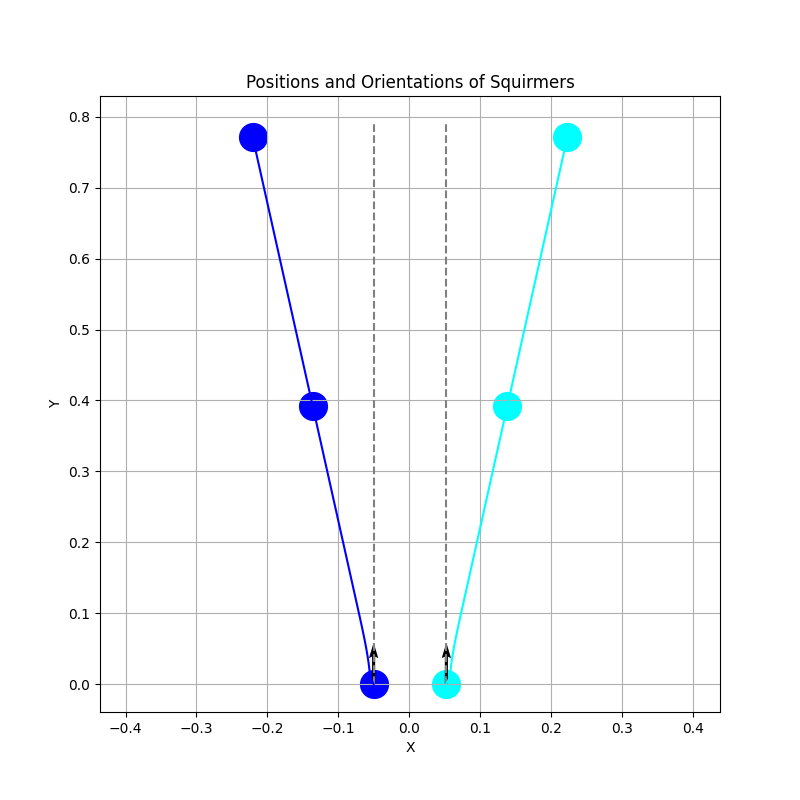
\includegraphics[width=1.1\textwidth]{graphs/simulations/sim_sq_sq/betam3/pi_2_.png}
        \caption{\footnotesize $\beta = -3$}
    \end{minipage}
    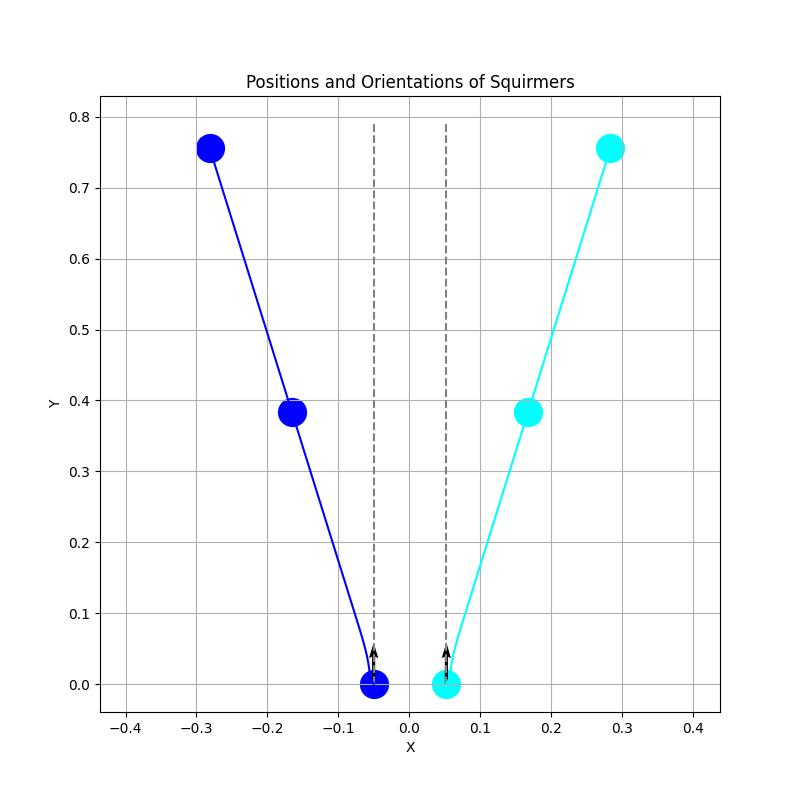
\includegraphics[width=0.55\textwidth]{graphs/simulations/sim_sq_sq/beta0/pi_2_.png}
    \caption{\footnotesize $\beta = 0$}
    Simulation parameters: radius $a=0.05$, velocity $v_0=1$, simulation time $T=0.8$\\
        position and orientation of squirmer1: $(x_1,y_1)=(-a,0)$, $\theta_1=\frac{\pi}{2}$,\\
        position and orientation of squirmer2: $(x_2,y_2)=(\frac{2a}{1.9},0)$, $\theta_2=\frac{\pi}{2}$
 \end{figure}
One can observe that their orientation changes due to the lubrification and steric forces which are applied on them. 
Those forces allow avoiding the overlapping of the two particles.\\
Each squirmer gradually distances itself from the other, consistent with the study \cite{Stark}.
For $\beta = 3$ the squirmers end the simulation at $x_1 = -0.35$ and $x_2 = 0.35$.
For $\beta = -3$ the squirmers end the simulation at $x_1 = -0.22$ and $x_2 = 0.22$.
 For $\beta = 0$ the squirmers end the simulation at $x_1 = -0.28$ and $x_2 = 0.28$.
 It is noteworthy that larger values of $\beta$ result in stronger forces and torques that push the
 squirmers further apart when both squirmers have an orientation $\theta = \frac{\pi}{2}$.
 \begin{figure}[H]
    \centering
    \textbf{$\theta_2 = \frac{3\pi}{4}$}\par\medskip
    \begin{minipage}{0.49\textwidth}
        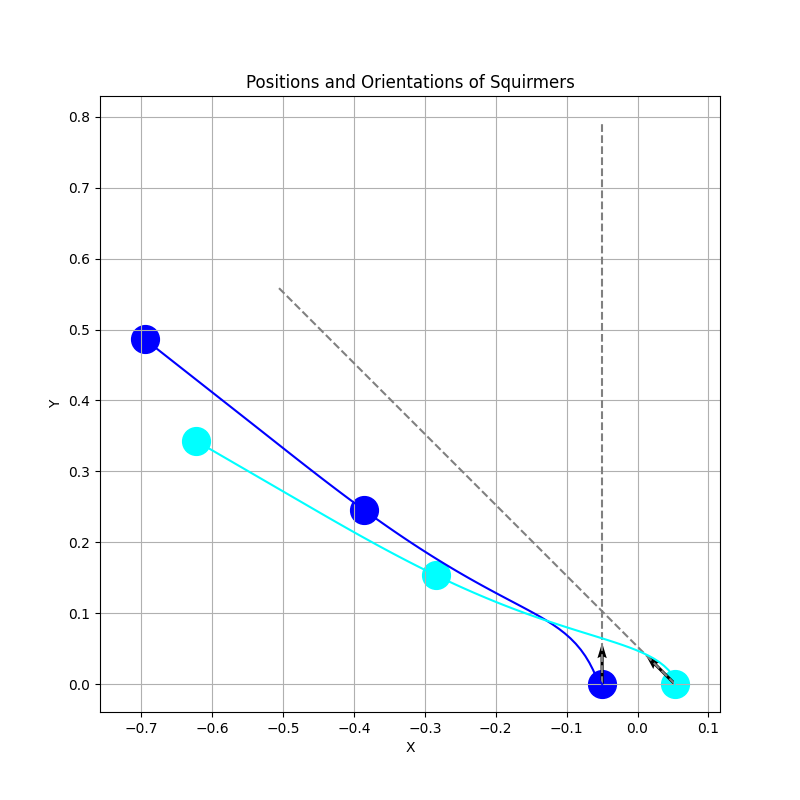
\includegraphics[width=1.1\textwidth]{graphs/simulations/sim_sq_sq/beta1_5/3pi_4_.png}
        \caption{\footnotesize $\beta = 1.5$}
    \end{minipage}\hfill
    \begin{minipage}{0.49\textwidth}
        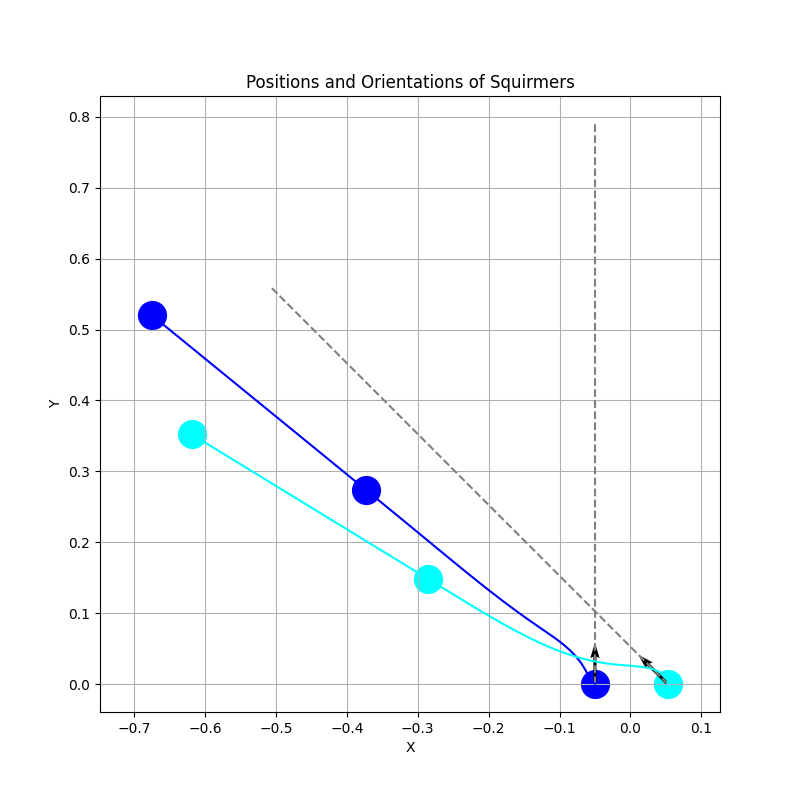
\includegraphics[width=1.1\textwidth]{graphs/simulations/sim_sq_sq/beta3/3pi_4_.png}
        \caption{\footnotesize $\beta = 3$}
    \end{minipage}
    \begin{minipage}{0.49\textwidth}
        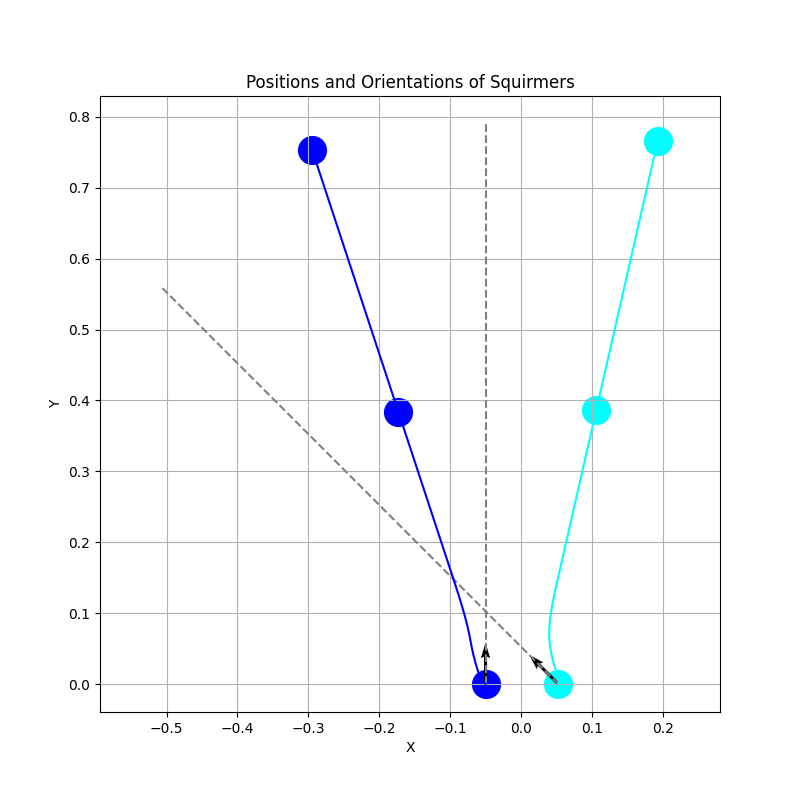
\includegraphics[width=1.1\textwidth]{graphs/simulations/sim_sq_sq/betam1_5/3pi_4_.png}
        \caption{\footnotesize $\beta = -1.5$}
    \end{minipage}\hfill
    \begin{minipage}{0.49\textwidth}
        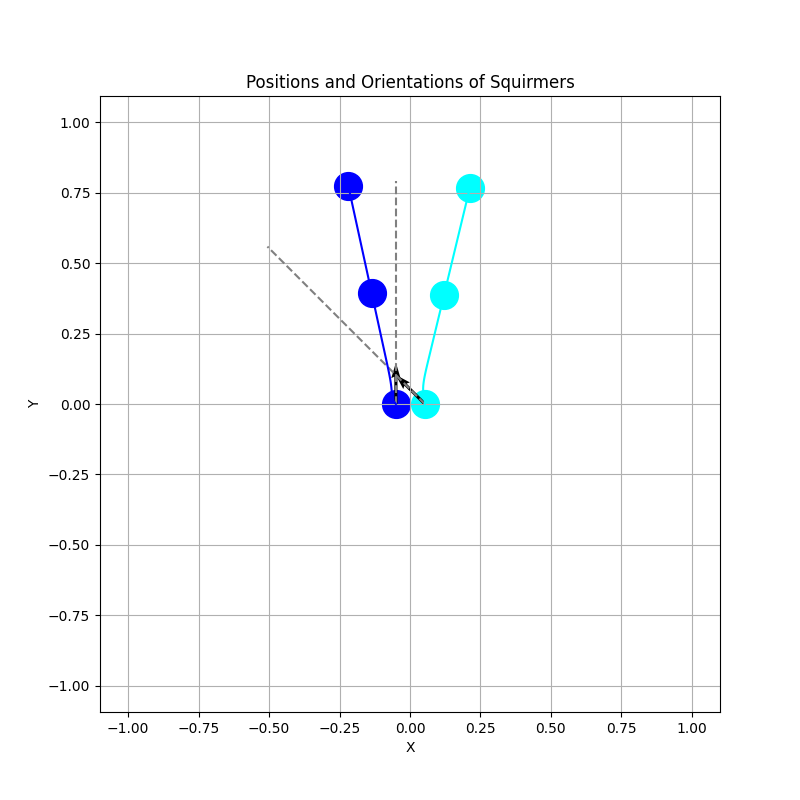
\includegraphics[width=1.1\textwidth]{graphs/simulations/sim_sq_sq/betam3/3pi_4_.png}
        \caption{\footnotesize $\beta = -3$}
    \end{minipage}
\end{figure}
\begin{figure}[H]
    \centering
    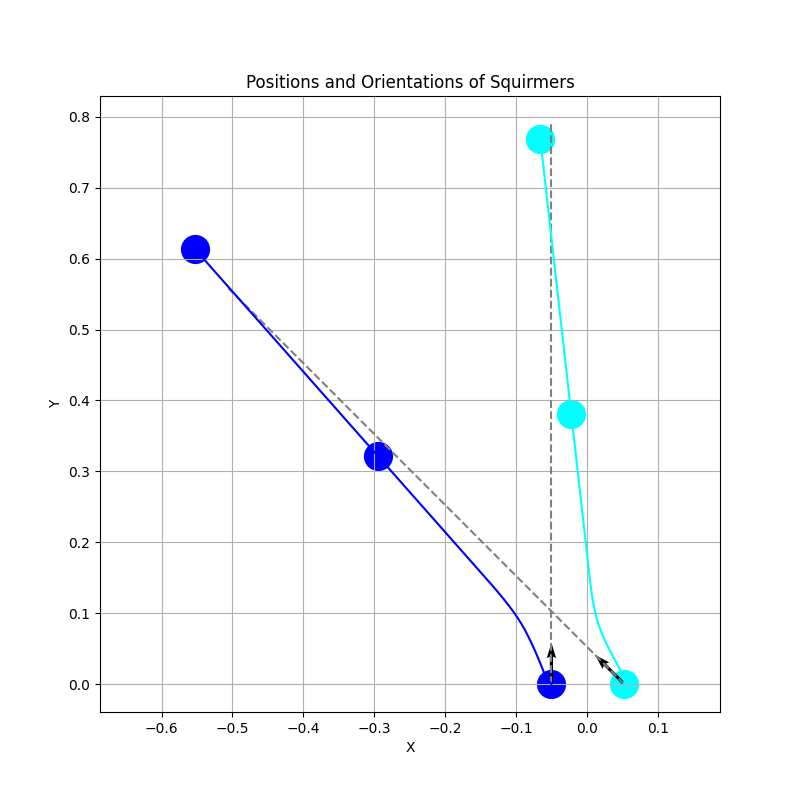
\includegraphics[width=0.55\textwidth]{graphs/simulations/sim_sq_sq/beta0/3pi_4_.png}
    \caption{\footnotesize $\beta = 0$}
\end{figure}
\begin{center}
    Simulation parameters: radius $a=0.05$, velocity $v_0=1$, simulation time $T=0.8$\\
        position and orientation of squirmer1: $(x_1,y_1)=(-a,0)$, $\theta_1=\frac{\pi}{2}$,\\
        position and orientation of squirmer2: $(x_2,y_2)=(\frac{2a}{1.9},0)$, $\theta_2=\frac{3\pi}{4}$
\end{center}
Our results are consistent with the previous study\cite{Stark} for $\beta = 0$. However, for $\beta > 0$ the right 
squirmer is attracted towards the left one,
 which is not consistent with the previous study. For $\beta < 0$ the torques on the right squirmer push
it away from the left one, also deviating with the previous study.\\
It is observed that for $\beta = 3$ the forces and torques pull the right squirmer towards the left one more strongly than for $\beta=1.5$.
Conversely, for $\beta = -3$ the right squirmer is pushed further away from the left one compared to $\beta = -1.5$.\\
In summary, for $\theta_2 = \frac{3\pi}{4}$, as $\beta$ increases, the right squirmer is more strongly pulled towards the left one. Conversely, as
$\beta$ decreases, the right squirmer is more strongly pushed away from the left one.


\begin{figure}[H]
    \centering
    \textbf{$\theta_2 = \pi$}\par\medskip
    \begin{minipage}{0.49\textwidth}
        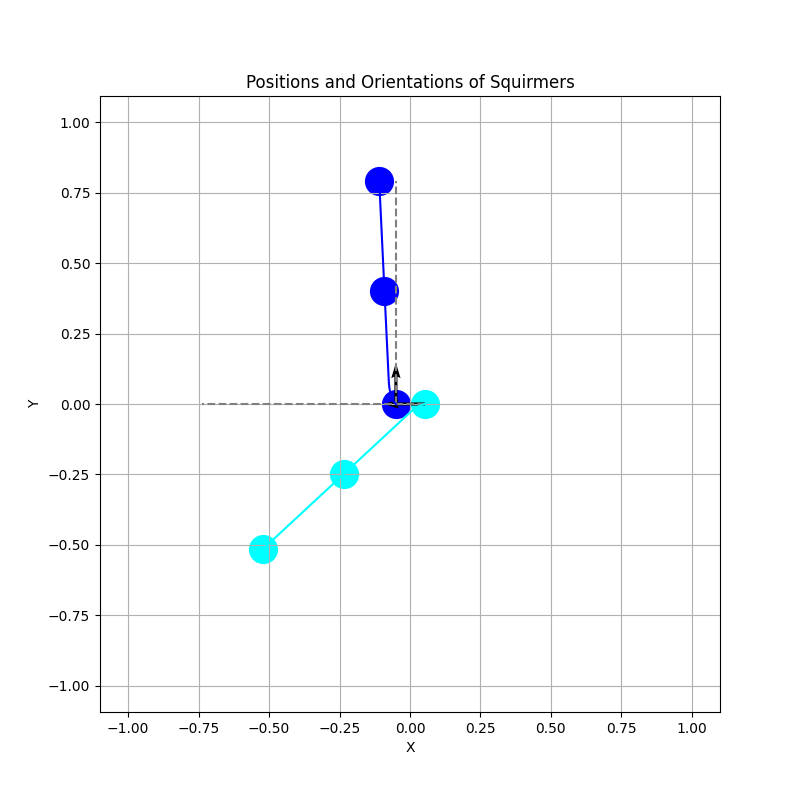
\includegraphics[width=1.1\textwidth]{graphs/simulations/sim_sq_sq/betam3/pi_.png}
        \caption{\footnotesize $\beta = -3$}
    \end{minipage}\hfill
    \begin{minipage}{0.49\textwidth}
        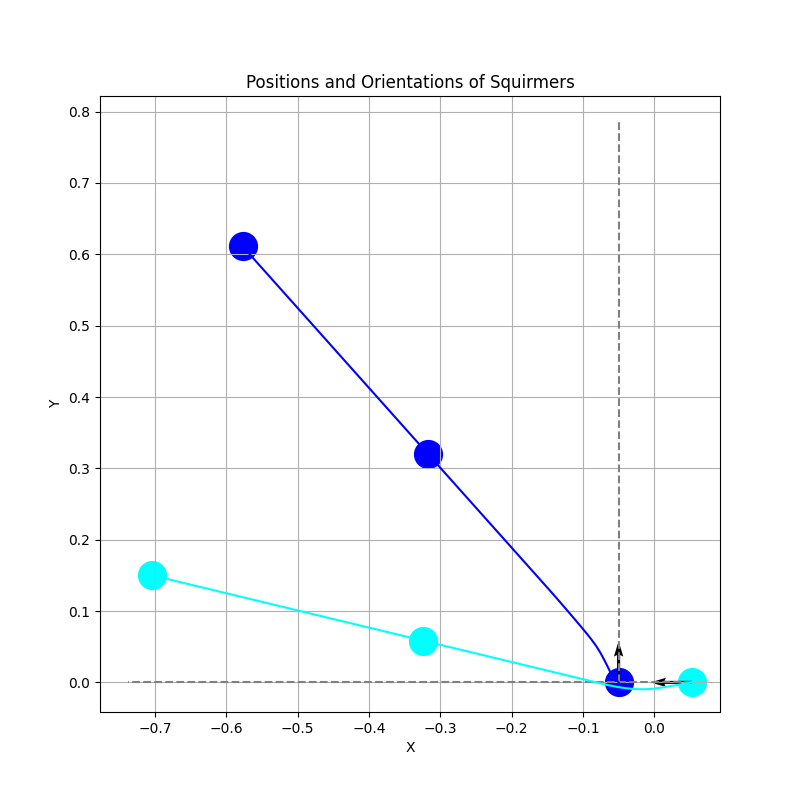
\includegraphics[width=1.1\textwidth]{graphs/simulations/sim_sq_sq/beta3/pi_.png}
        \caption{\footnotesize $\beta = 3$}
    \end{minipage}
    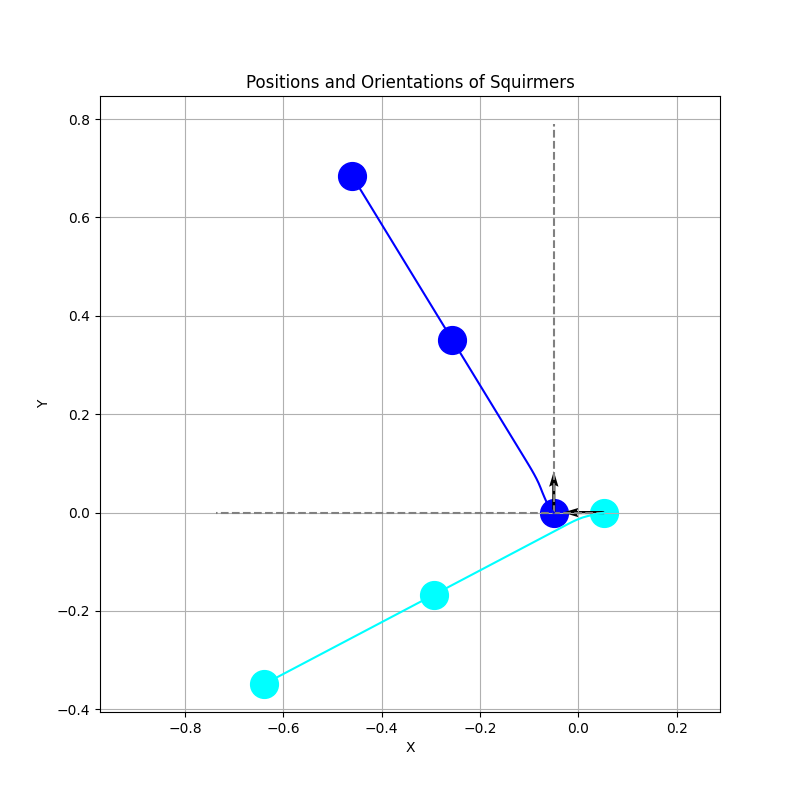
\includegraphics[width=0.55\textwidth]{graphs/simulations/sim_sq_sq/beta0/pi_.png}
    \caption{\footnotesize $\beta = 0$}
    Simulation parameters: radius $a=0.05$, velocity $v_0=1$, simulation time $T=0.8$\\
        position and orientation of squirmer1: $(x_1,y_1)=(-a,0)$, $\theta_1=\frac{\pi}{2}$,\\
        position and orientation of squirmer2: $(x_2,y_2)=(\frac{2a}{1.9},0)$, $\theta_2=\pi$
\end{figure}
Our results are not consistent with the previous study\cite{Stark}. Our results shows that the right squirmer's position
and orientation are altered by the forces and torques for any $\beta$ while the previous study showed that the right squirmer's
orientation is not supposed to change.

\begin{figure}
    \centering
    \begin{minipage}{0.49\textwidth}
        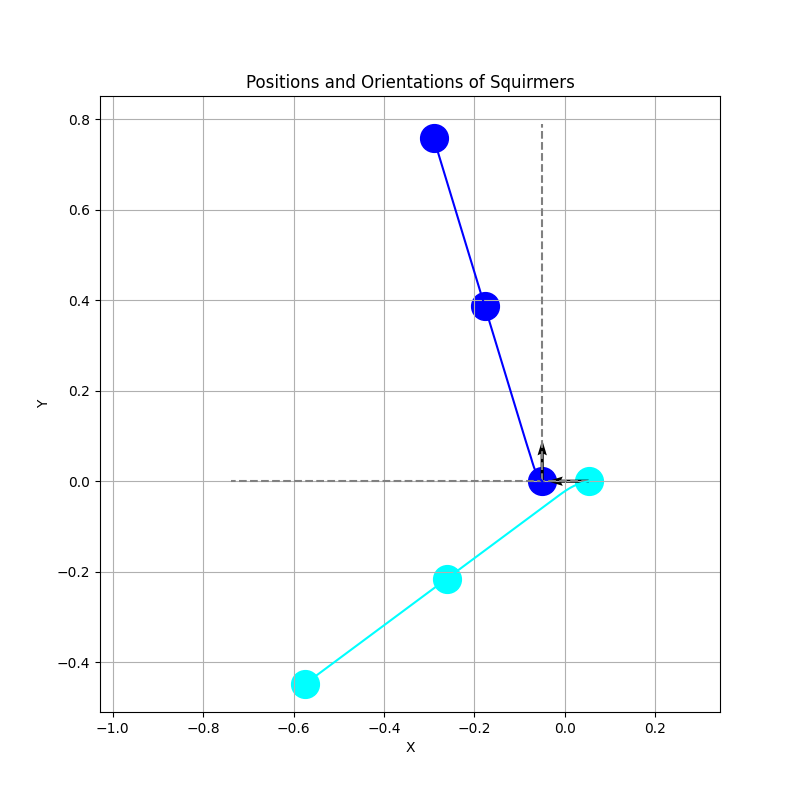
\includegraphics[width=1.1\textwidth]{graphs/simulations/sim_sq_sq/betam1_5/pi_.png}
        \caption{\footnotesize $\beta = -1.5$}
    \end{minipage}\hfill
    \begin{minipage}{0.49\textwidth}
        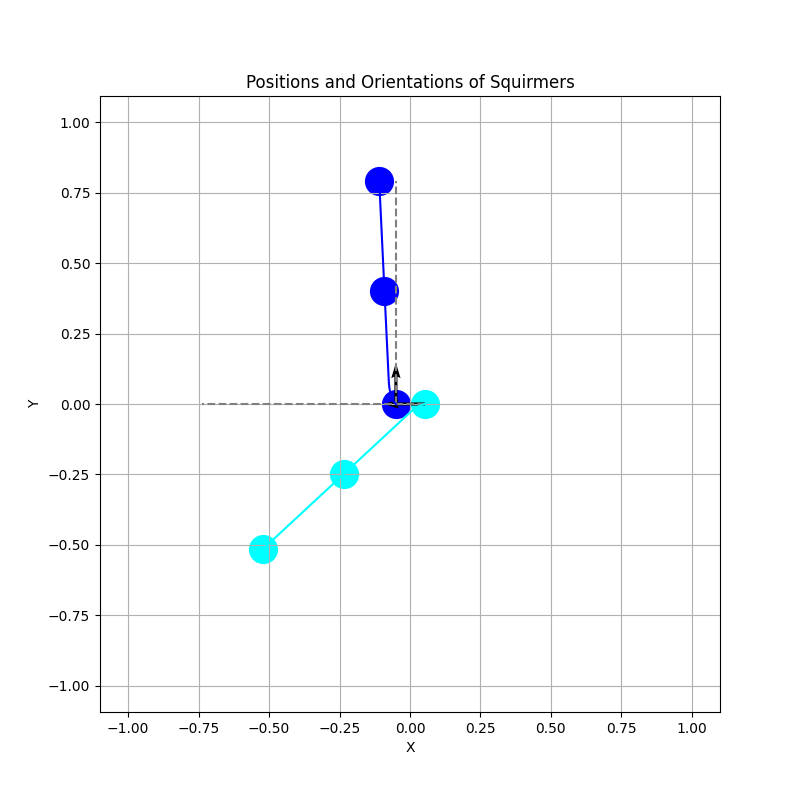
\includegraphics[width=1.1\textwidth]{graphs/simulations/sim_sq_sq/betam3/pi_.png}
        \caption{\footnotesize $\beta = -3$}
    \end{minipage}
    \begin{minipage}{0.49\textwidth}
        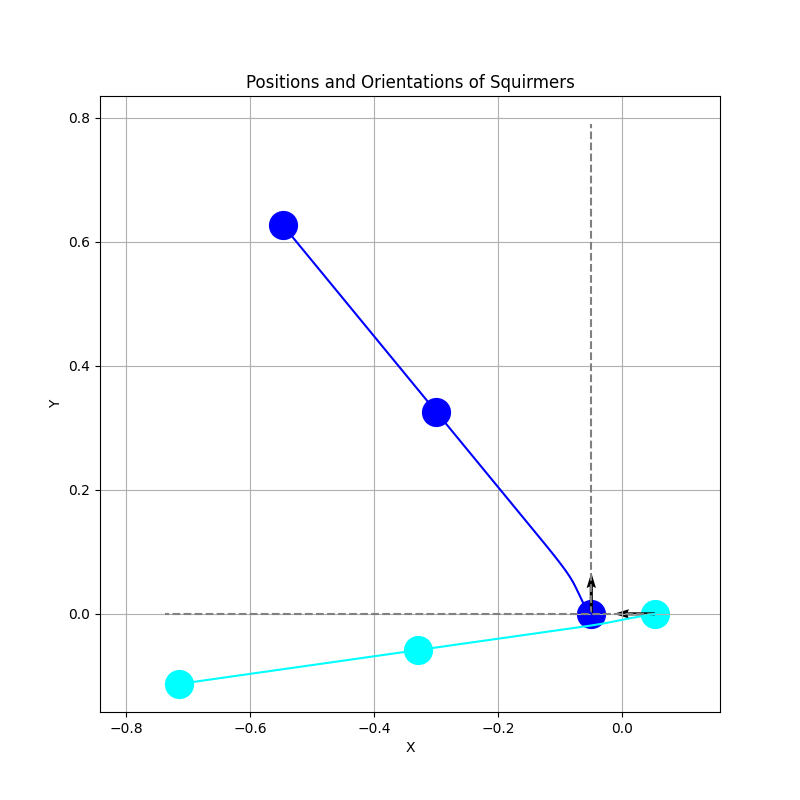
\includegraphics[width=1.1\textwidth]{graphs/simulations/sim_sq_sq/beta1_5/pi_.png}
        \caption{\footnotesize $\beta = 1.5$}
    \end{minipage}\hfill
    \begin{minipage}{0.49\textwidth}
        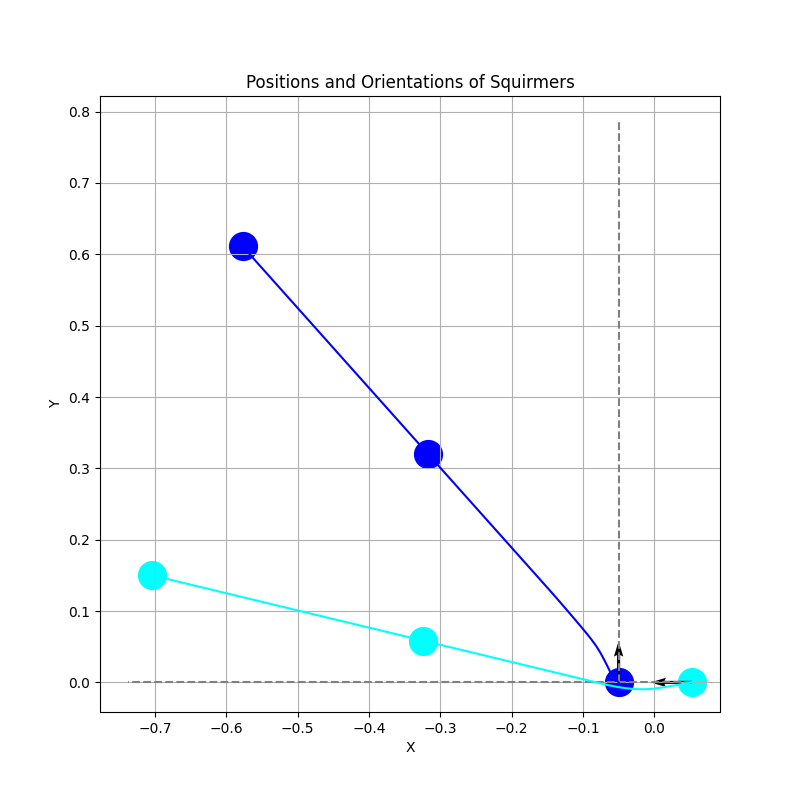
\includegraphics[width=1.1\textwidth]{graphs/simulations/sim_sq_sq/beta3/pi_.png}
        \caption{\footnotesize $\beta = 3$}
    \end{minipage}
    Simulation parameters: radius $a=0.05$, velocity $v_0=1$, simulation time $T=0.8$\\
        position and orientation of squirmer1: $(x_1,y_1)=(-a,0)$, $\theta_1=\frac{\pi}{2}$,\\
        position and orientation of squirmer2: $(x_2,y_2)=(\frac{2a}{1.9},0)$, $\theta_2=\pi$
\end{figure}
For $\beta = -3$, the orientation at the end of the simulation is less altered compared to $\beta = -1.5$.
For $\beta = 3$, the right squirmer ands up behind the left one, whereas for $\beta = 1.5$, the right
squirmer is pushed away.
Our results indicate that for $\theta_2 = \pi$, as $\beta$ increases, the right squirmer is more strongly pulled 
towards the left one, while as $\beta$ decreases, the torques acting on the left squirmer also decrease.

\begin{figure}[H]
    \centering
    \textbf{$\theta_2 = -\frac{3\pi}{4}$}\par\medskip
    \begin{minipage}{0.49\textwidth}
        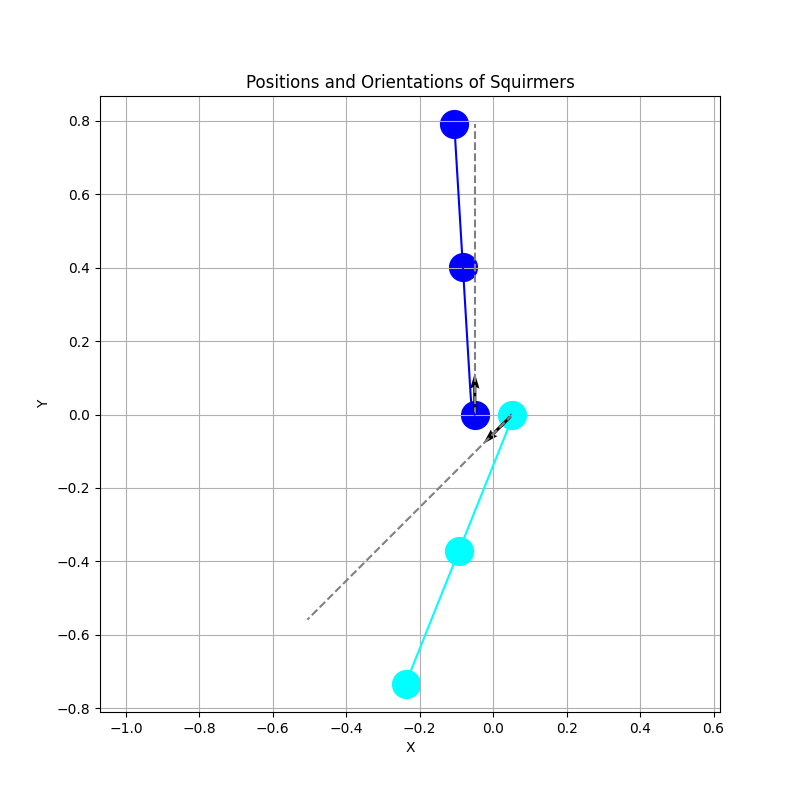
\includegraphics[width=1.1\textwidth]{graphs/simulations/sim_sq_sq/betam3/m3pi_4_.png}
        \caption{\footnotesize $\beta = -3$}
    \end{minipage}\hfill
    \begin{minipage}{0.49\textwidth}
        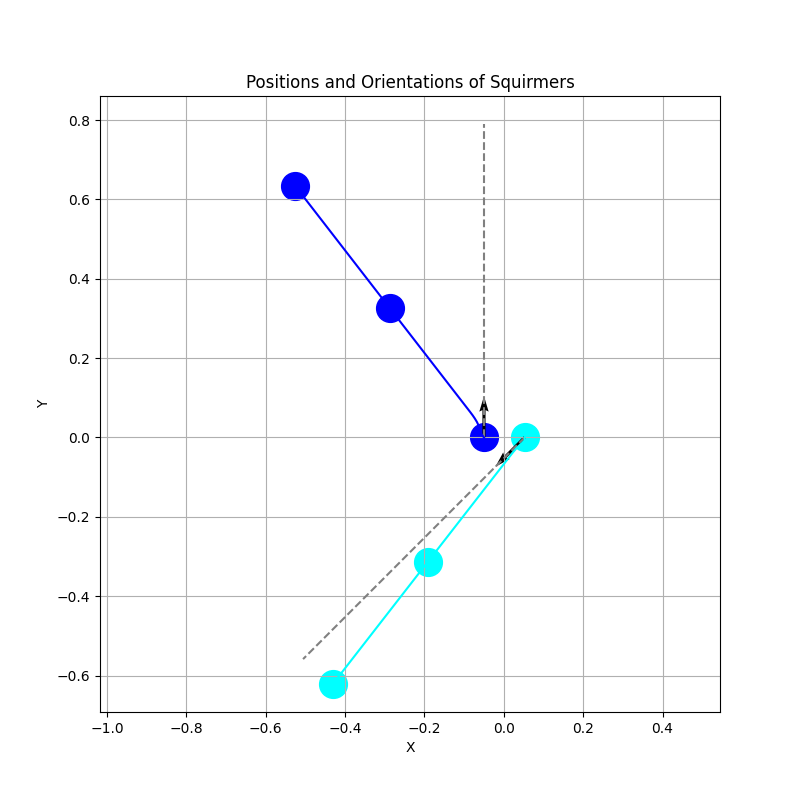
\includegraphics[width=1.1\textwidth]{graphs/simulations/sim_sq_sq/beta3/m3pi_4_.png}
        \caption{\footnotesize $\beta = 3$}
    \end{minipage}
    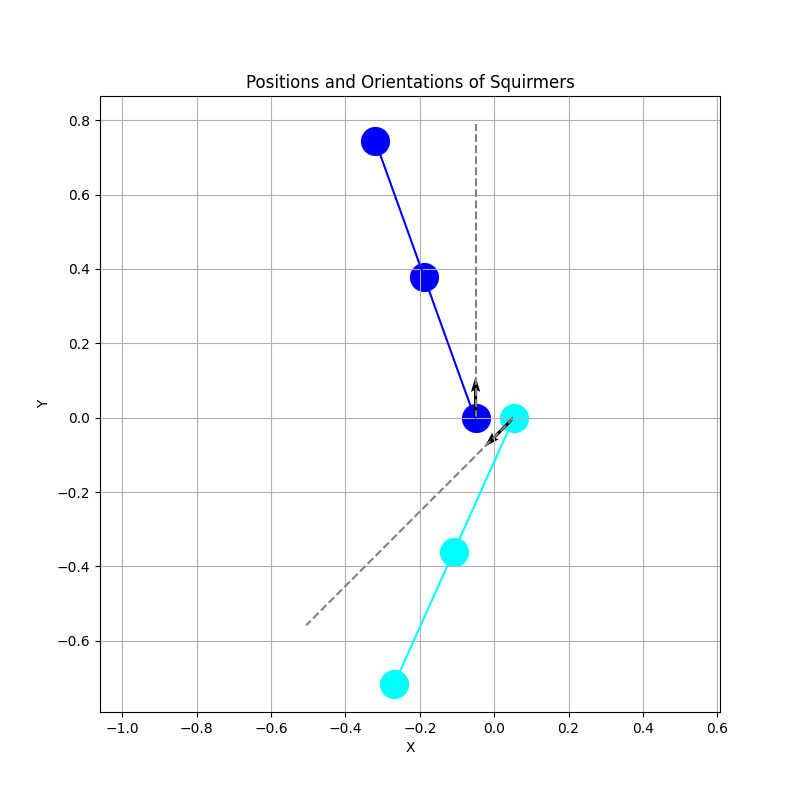
\includegraphics[width=0.55\textwidth]{graphs/simulations/sim_sq_sq/beta0/m3pi_4_.png}
    \caption{\footnotesize $\beta = 0$}
\end{figure}
\begin{center}
    Simulation parameters: radius $a=0.05$, velocity $v_0=1$, simulation time $T=0.8$\\
        position and orientation of squirmer1: $(x_1,y_1)=(-a,0)$, $\theta_1=\frac{\pi}{2}$,\\
        position and orientation of squirmer2: $(x_2,y_2)=(\frac{2a}{1.9},0)$, $\theta_2=-\frac{3\pi}{4}$
\end{center}
Our results are consistent with the previous study\cite{Stark} for $\beta \ge 0$ as the torques acting on the right squirmer
are weaker than the ones acting on the left one. On the contrary, for $\beta < 0$ the torques acting on the right squirmer are larger
than the ones acting on the left one.

\begin{figure}[H]
    \centering
    \textbf{$\theta_2 = -\frac{\pi}{2}$}\par\medskip
    \begin{minipage}{0.49\textwidth}
        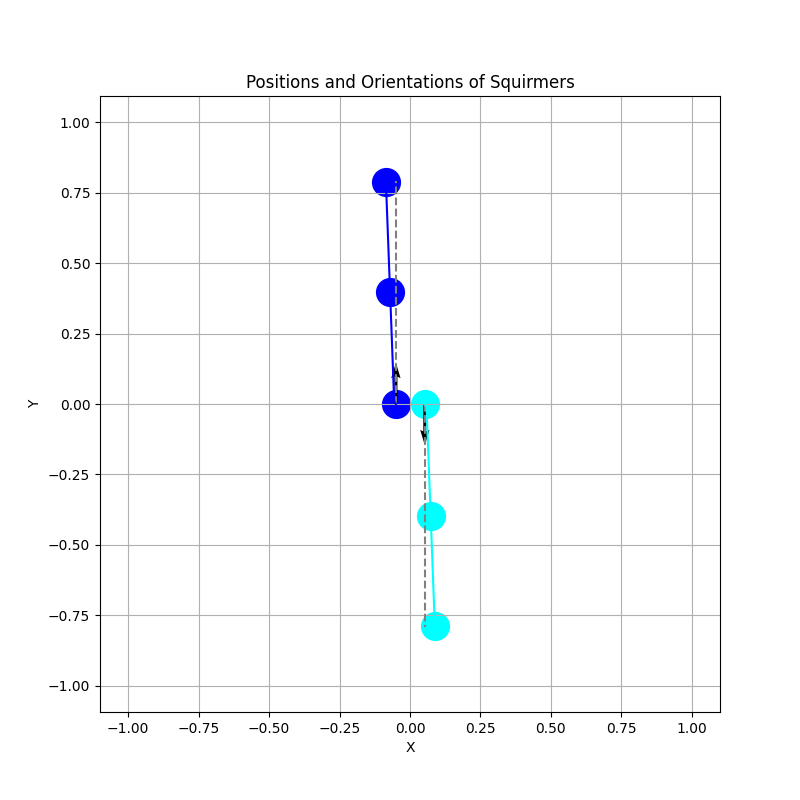
\includegraphics[width=1.1\textwidth]{graphs/simulations/sim_sq_sq/betam3/mpi_2_.png}
        \caption{\footnotesize $\beta = -3$}
    \end{minipage}\hfill
    \begin{minipage}{0.49\textwidth}
        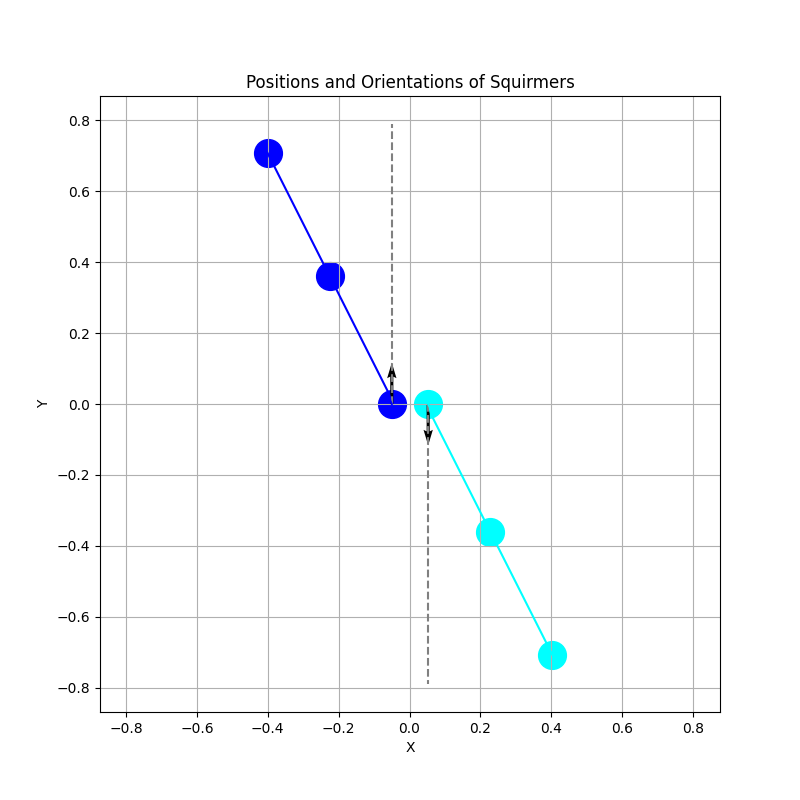
\includegraphics[width=1.1\textwidth]{graphs/simulations/sim_sq_sq/beta3/mpi_2_.png}
        \caption{\footnotesize $\beta = 3$}
    \end{minipage}
    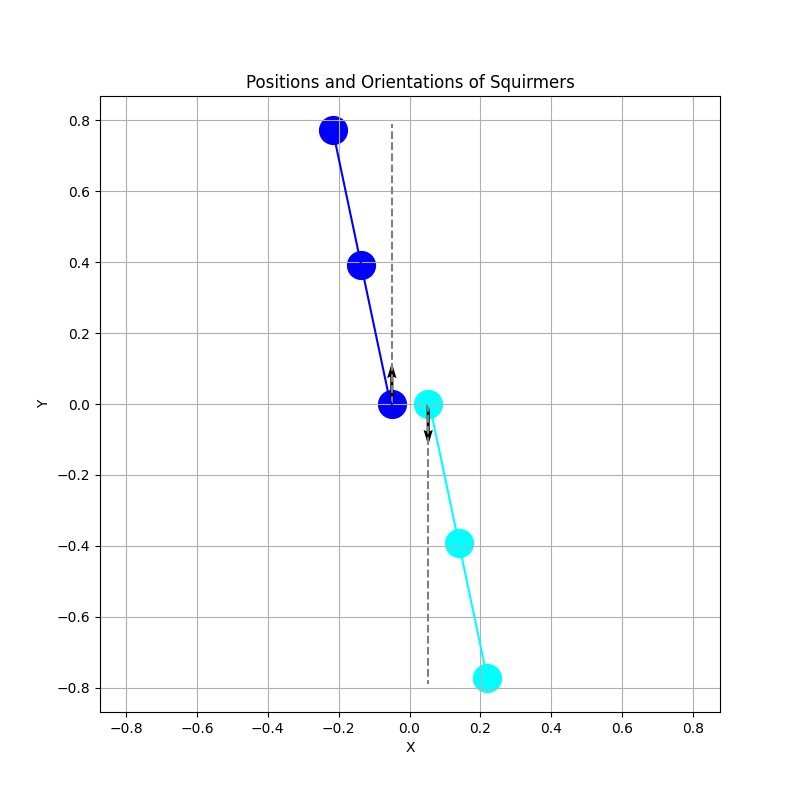
\includegraphics[width=0.55\textwidth]{graphs/simulations/sim_sq_sq/beta0/mpi_2_.png}
    \caption{\footnotesize $\beta = 0$}
\end{figure}
\begin{center}
    Simulation parameters: radius $a=0.05$, velocity $v_0=1$, simulation time $T=0.8$\\
        position and orientation of squirmer1: $(x_1,y_1)=(-a,0)$, $\theta_1=\frac{\pi}{2}$,\\
        position and orientation of squirmer2: $(x_2,y_2)=(\frac{2a}{1.9},0)$, $\theta_2=-\frac{\pi}{2}$
\end{center}
Our results are consistent with the previous study\cite{Stark} as the torques acting on the right squirmer are equal to
those acting on the left squirmer for all values of $\beta$.

\begin{figure}[H]
    \centering
    \textbf{$\theta_2 = -\frac{\pi}{4}$}\par\medskip
    \begin{minipage}{0.49\textwidth}
        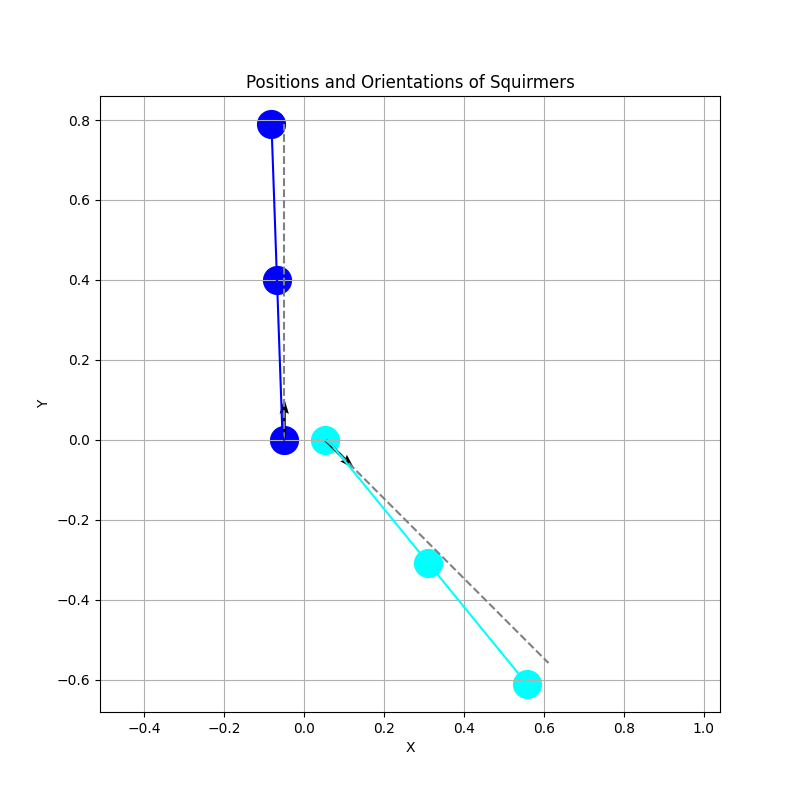
\includegraphics[width=1.1\textwidth]{graphs/simulations/sim_sq_sq/betam3/mpi_4_.png}
        \caption{\footnotesize $\beta = -3$}
    \end{minipage}\hfill
    \begin{minipage}{0.49\textwidth}
        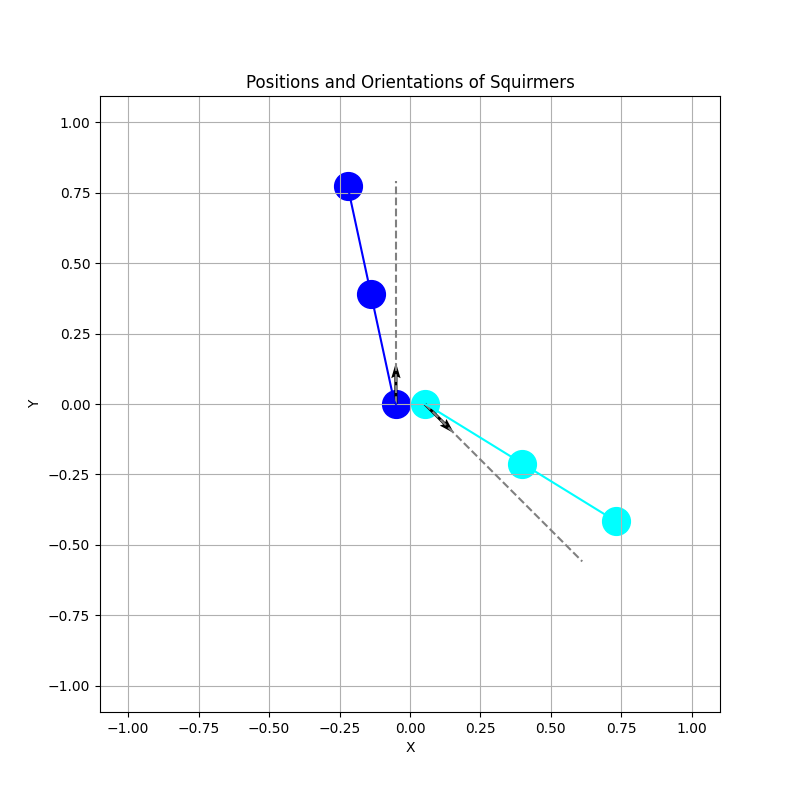
\includegraphics[width=1.1\textwidth]{graphs/simulations/sim_sq_sq/beta3/mpi_4_.png}
        \caption{\footnotesize $\beta = 3$}
    \end{minipage}
    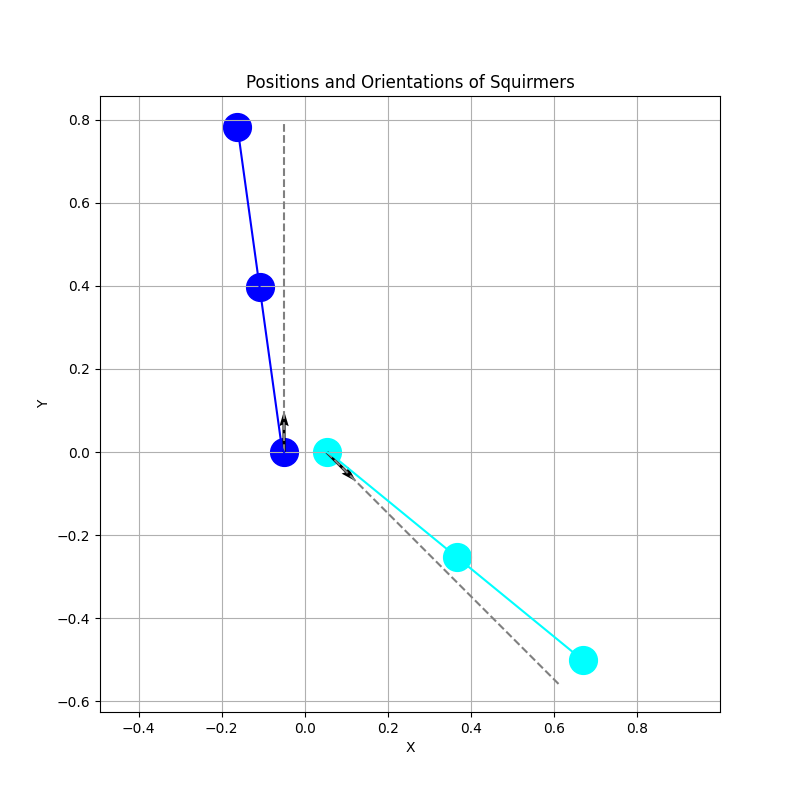
\includegraphics[width=0.55\textwidth]{graphs/simulations/sim_sq_sq/beta0/mpi_4_.png}
    \caption{\footnotesize $\beta = 0$}
\end{figure}
\begin{center}
    Simulation parameters: radius $a=0.05$, velocity $v_0=1$, simulation time $T=0.8$\\
        position and orientation of squirmer1: $(x_1,y_1)=(-a,0)$, $\theta_1=\frac{\pi}{2}$,\\
        position and orientation of squirmer2: $(x_2,y_2)=(\frac{2a}{1.9},0)$, $\theta_2=-\frac{\pi}{4}$
\end{center}
Our results are consistent with the previous study\cite{Stark} for $\beta = 0$ as the torques acting on the right 
squirmer are weaker to those acting on the left squirmer. For $\beta = 3$ the torques acting on the right squirmer are
equal to the those acting on the left squirmer which does not align with the previous study.
For $\beta = -3$ the rotation vector does not align with the previous study.
\\
\\
\begin{figure}[H]
    \centering
    \textbf{$\theta_2 = \frac{\pi}{4}$}\par\medskip
    \begin{minipage}{0.49\textwidth}
        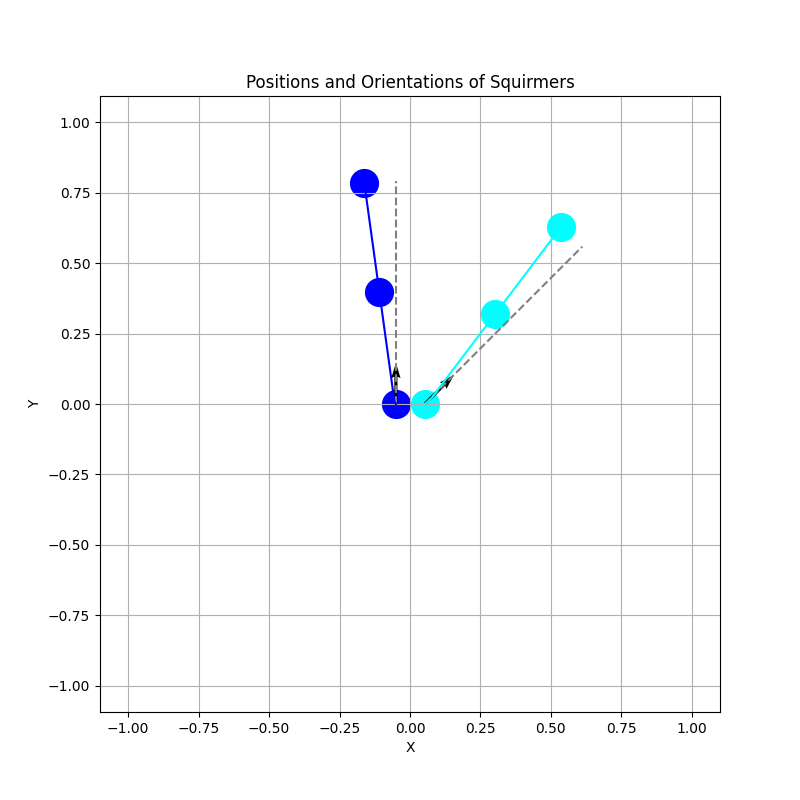
\includegraphics[width=1.1\textwidth]{graphs/simulations/sim_sq_sq/betam3/pi_4_.png}
        \caption{\footnotesize $\beta = -3$}
    \end{minipage}\hfill
    \begin{minipage}{0.49\textwidth}
        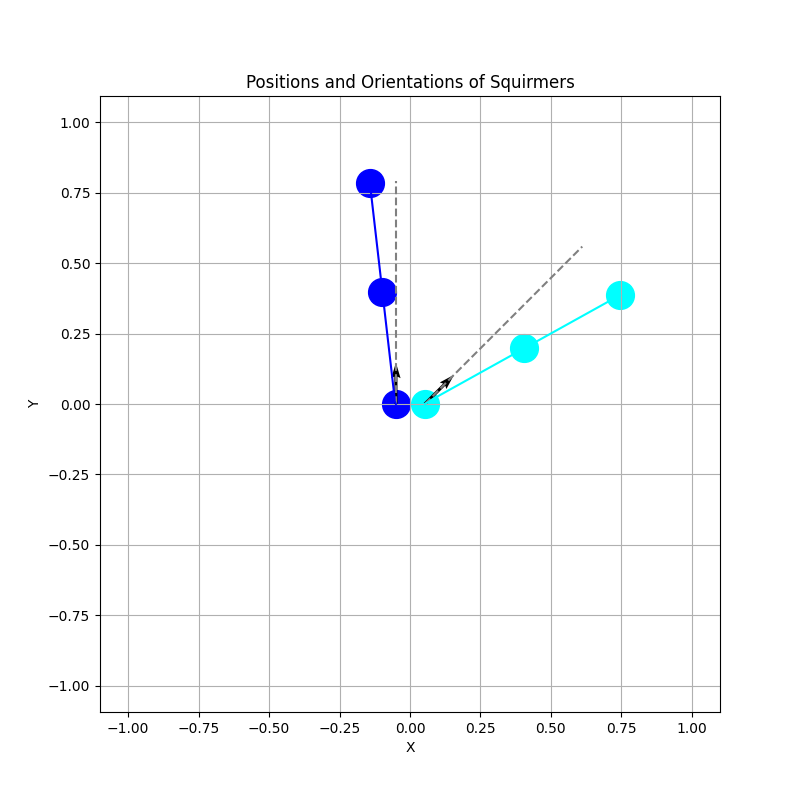
\includegraphics[width=1.1\textwidth]{graphs/simulations/sim_sq_sq/beta3/pi_4_.png}
        \caption{\footnotesize $\beta = 3$}
    \end{minipage}
\end{figure}
\begin{figure}[H]
    \centering
    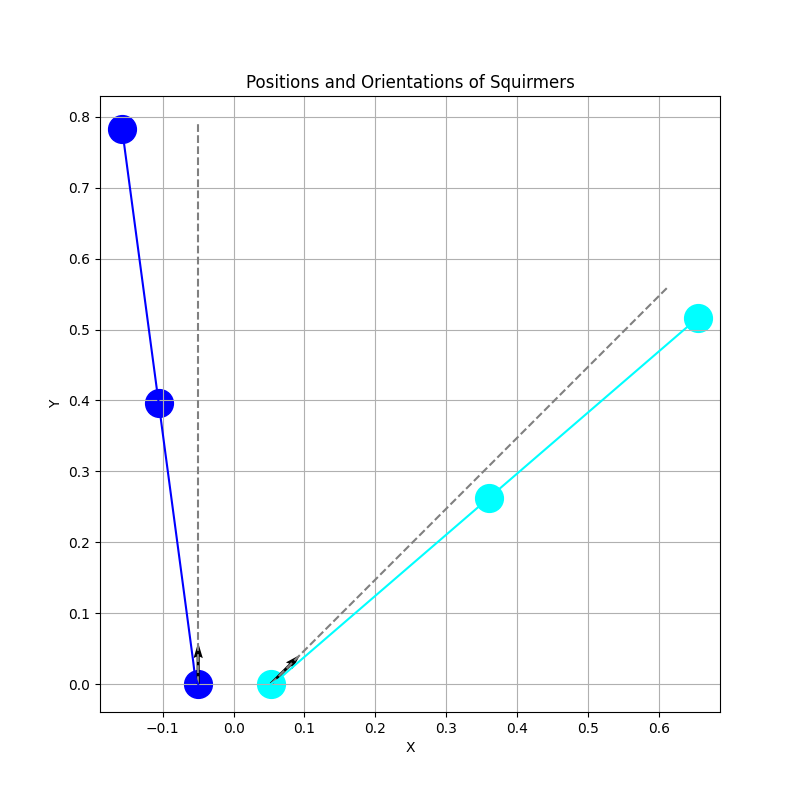
\includegraphics[width=0.55\textwidth]{graphs/simulations/sim_sq_sq/beta0/pi_4_.png}
    \caption{\footnotesize $\beta = 0$}
\end{figure}
\begin{center}
    Simulation parameters: radius $a=0.05$, velocity $v_0=1$, simulation time $T=0.8$\\
        position and orientation of squirmer1: $(x_1,y_1)=(-a,0)$, $\theta_1=\frac{\pi}{2}$,\\
        position and orientation of squirmer2: $(x_2,y_2)=(\frac{2a}{1.9},0)$, $\theta_2=\frac{\pi}{4}$
\end{center}
Our results are consistent with the previous study\cite{Stark} for $\beta = 0$ as the torques acting on the right 
squirmer are weaker to those acting on the left squirmer. For $\beta = 3$ the torques acting on the right squirmer are
greater to the those acting on the left squirmer, which does not align with the previous study.
For $\beta = -3$ the rotation vector does not align with the previous study.

\subsection{Simulation of squirmer-border interacting}
In this section twenty simulation of a squirmer near a border are conducted. The parameters of the simulations are fixed
except for the orientation and $\beta$ parameter. The squirmer is placed at $(x,y) = (-0.4,-0.7)$, has a radius of $a=0.05$,
a velocity $v_0=1$, an initial orientation $\theta$ varying among $-\frac{\pi}{6}$, $-\frac{\pi}{4}$, $-\frac{\pi}{3}$
and $-\frac{\pi}{2}$ and a $\beta$ value varying among $\beta_0 = 0, \beta_1 = 1.5, \beta_2 = 3, \beta_3 = -1.5, \beta_4 = -3$.\\
One can execute these simulations by running the command:
 \begin{verbatim}
    python Code/run.py border 1 filename
 \end{verbatim}
 The parameters can be changed in the \texttt{Code/run.py} and \texttt{Code/interactingsquirmers.py} files.\\
 We show the trajectory of the squirmer as well as his initial orientation. A red circle and the corresponding time are marked when the squirmer
 reaches or exceeds the original height. Circles are plotted at the start, 
 middle, and end of the simulation, with their radii proportional to the squirmer's size.
 \begin{figure}[H]
    \centering
    \textbf{$\theta = -\frac{\pi}{6}$}\par\medskip
    \begin{minipage}{0.49\textwidth}
        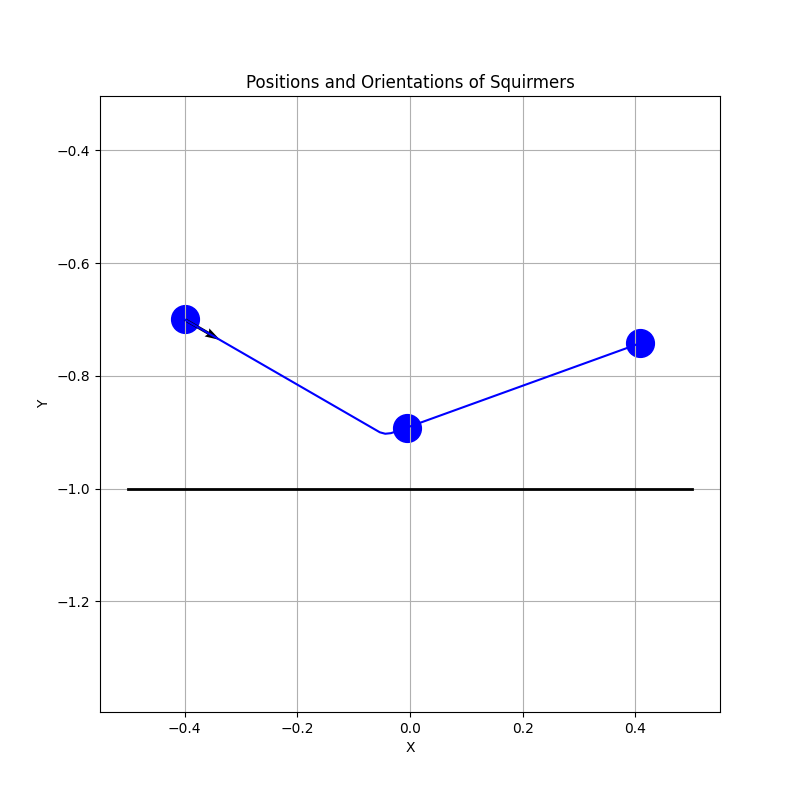
\includegraphics[width=1.1\textwidth]{graphs/simulations/border/beta1_5/mpi_6.png}
        \caption{\footnotesize $\beta = 1.5$}
    \end{minipage}\hfill
    \begin{minipage}{0.49\textwidth}
        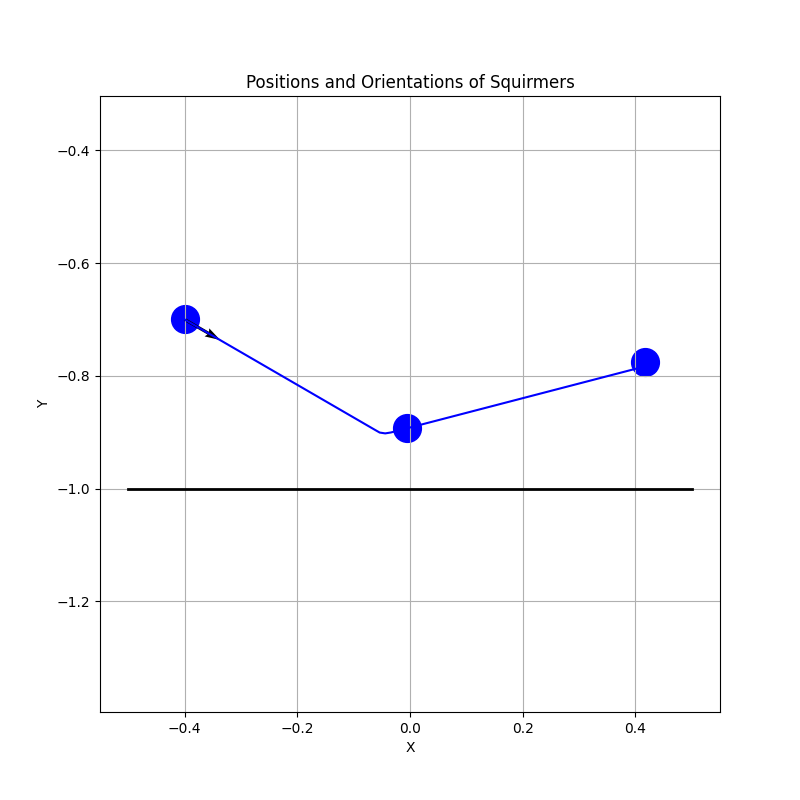
\includegraphics[width=1.1\textwidth]{graphs/simulations/border/beta3/mpi_6.png}
        \caption{\footnotesize $\beta = 3$}
    \end{minipage}
    \begin{minipage}{0.49\textwidth}
        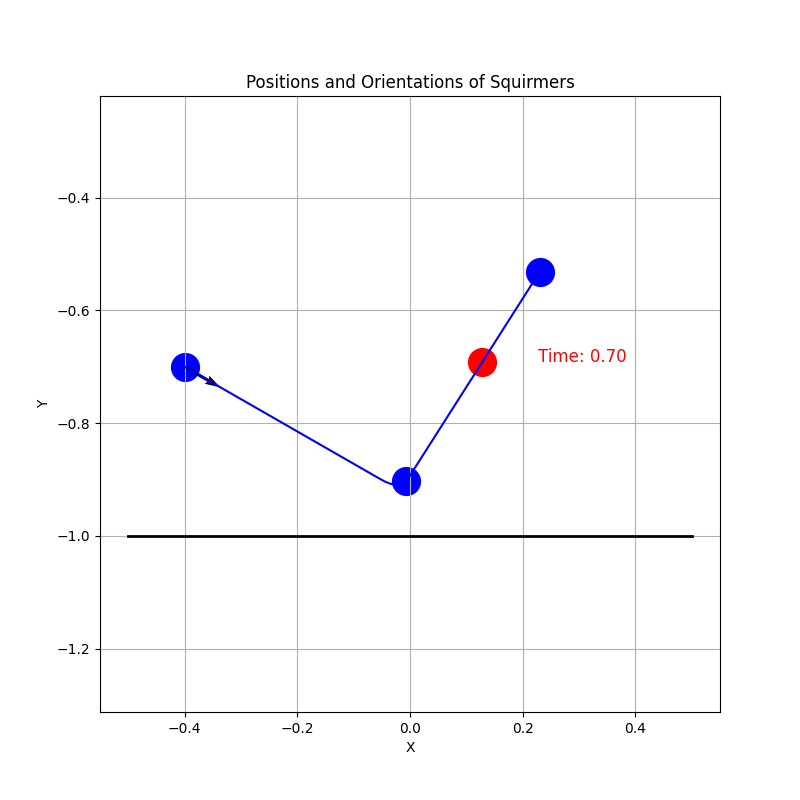
\includegraphics[width=1.1\textwidth]{graphs/simulations/border/betam1_5/mpi_6.png}
        \caption{\footnotesize $\beta = -1.5$}
    \end{minipage}\hfill
    \begin{minipage}{0.49\textwidth}
        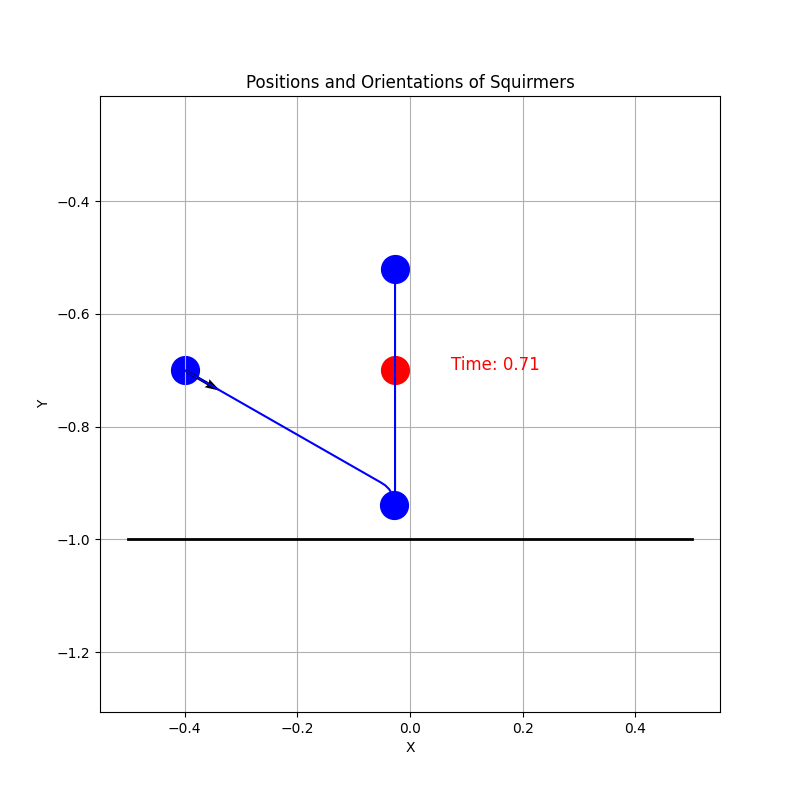
\includegraphics[width=1.1\textwidth]{graphs/simulations/border/betam3/mpi_6.png}
        \caption{\footnotesize $\beta = -3$}
    \end{minipage}
\end{figure}
\begin{figure}[H]
    \centering
    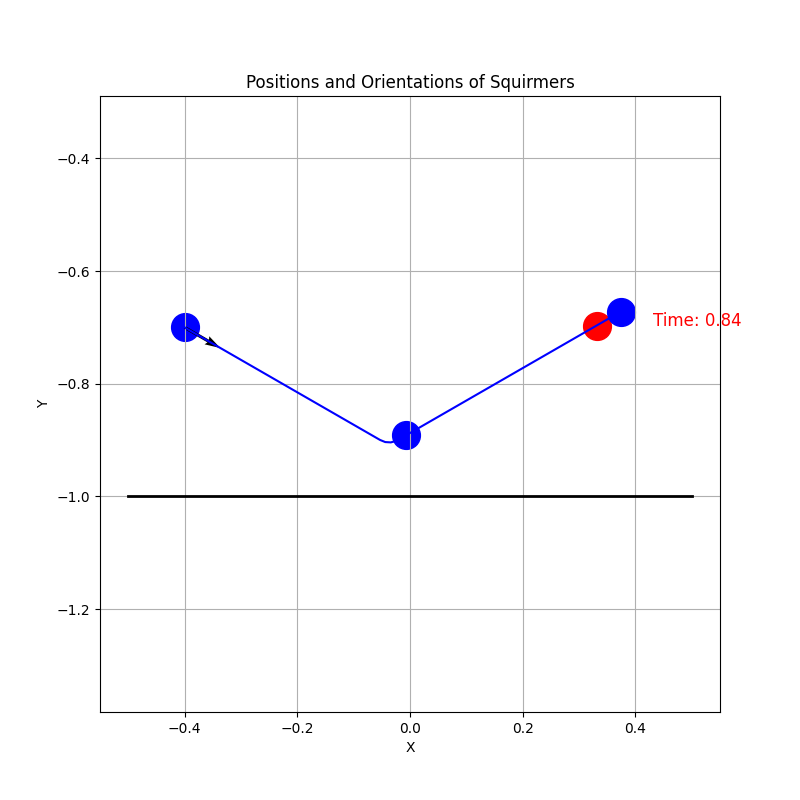
\includegraphics[width=0.55\textwidth]{graphs/simulations/border/beta0/mpi_6.png}
    \caption{\footnotesize $\beta = 0$}
    Simulation parameters: radius $a=0.05$, velocity $v_0=1$, simulation time $T=0.9$\\
        position and orientation of squirmer: $(x_1,y_1)=(-0.4,-0.7)$, $\theta=-\frac{\pi}{6}$
\end{figure}
Our results shows that for $\theta = -\frac{\pi}{6}$, as $\beta$ increases, the squirmer's orientation upon interaction becomes parallel to the border.
On the contrary, as $\beta$ decreases, the squirmer's orientation upon interaction becomes tangential to the border.\\
The fact that the orientation after interaction is tangential does not necessarily mean that the particle reaches the initial 
height more quickly, as observed when $\beta = -3$ compared to when $\beta = -1.5$.

\begin{figure}[H]
    \centering
    \textbf{$\theta = -\frac{\pi}{4}$}\par\medskip
    \begin{minipage}{0.49\textwidth}
        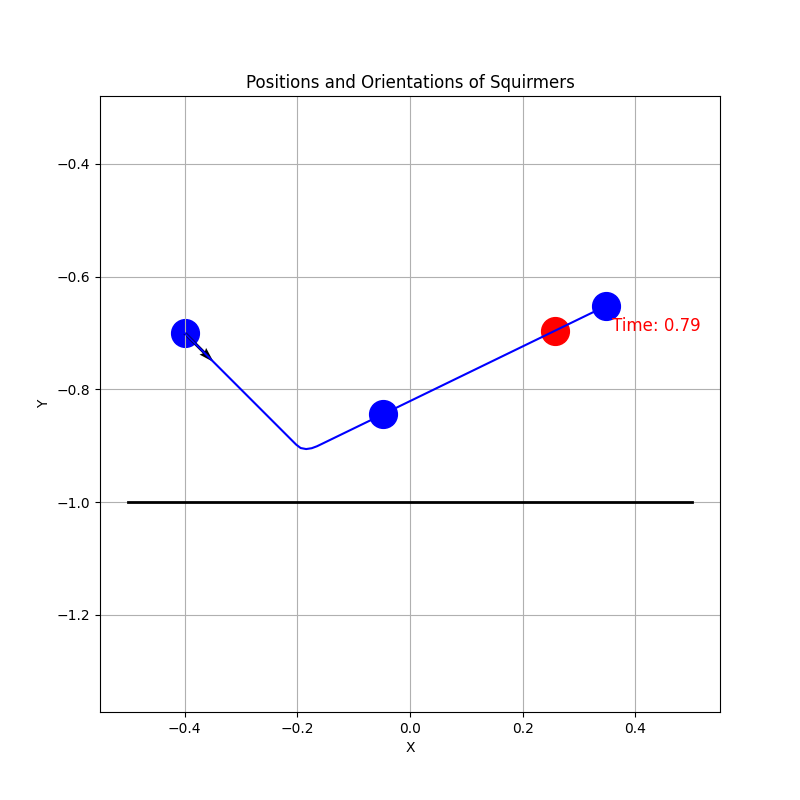
\includegraphics[width=1.1\textwidth]{graphs/simulations/border/beta1_5/mpi_4.png}
        \caption{\footnotesize $\beta = 1.5$}
    \end{minipage}\hfill
    \begin{minipage}{0.49\textwidth}
        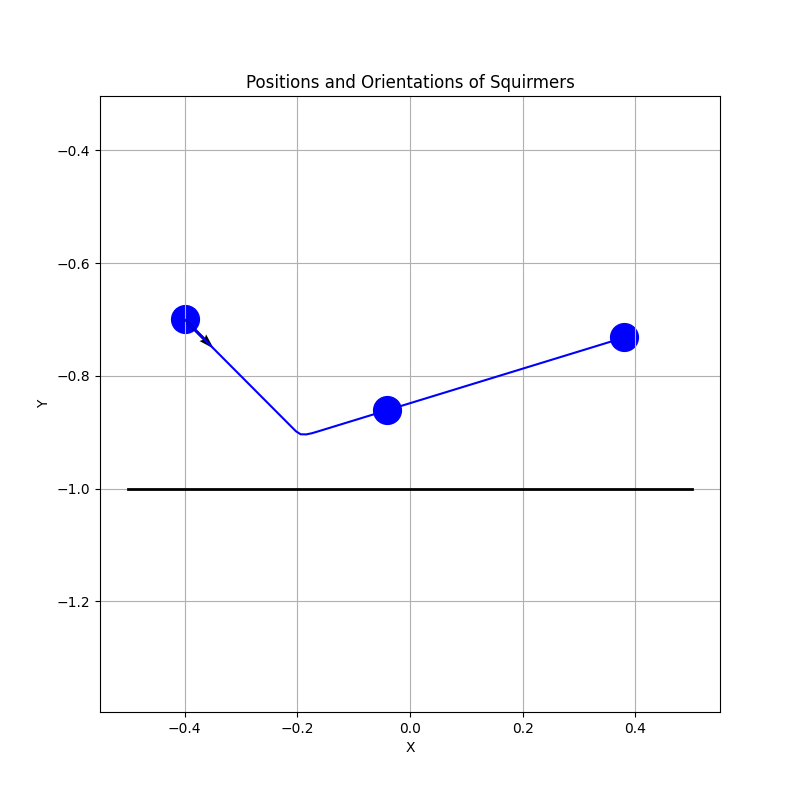
\includegraphics[width=1.1\textwidth]{graphs/simulations/border/beta3/mpi_4.png}
        \caption{\footnotesize $\beta = 3$}
    \end{minipage}
    \begin{minipage}{0.49\textwidth}
        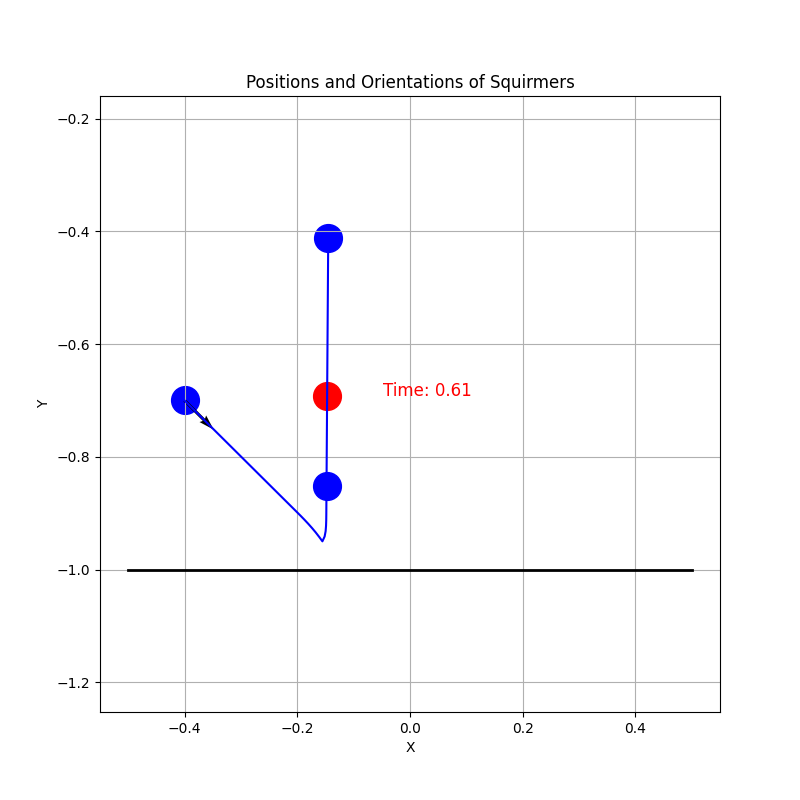
\includegraphics[width=1.1\textwidth]{graphs/simulations/border/betam1_5/mpi_4.png}
        \caption{\footnotesize $\beta = -1.5$}
    \end{minipage}\hfill
    \begin{minipage}{0.49\textwidth}
        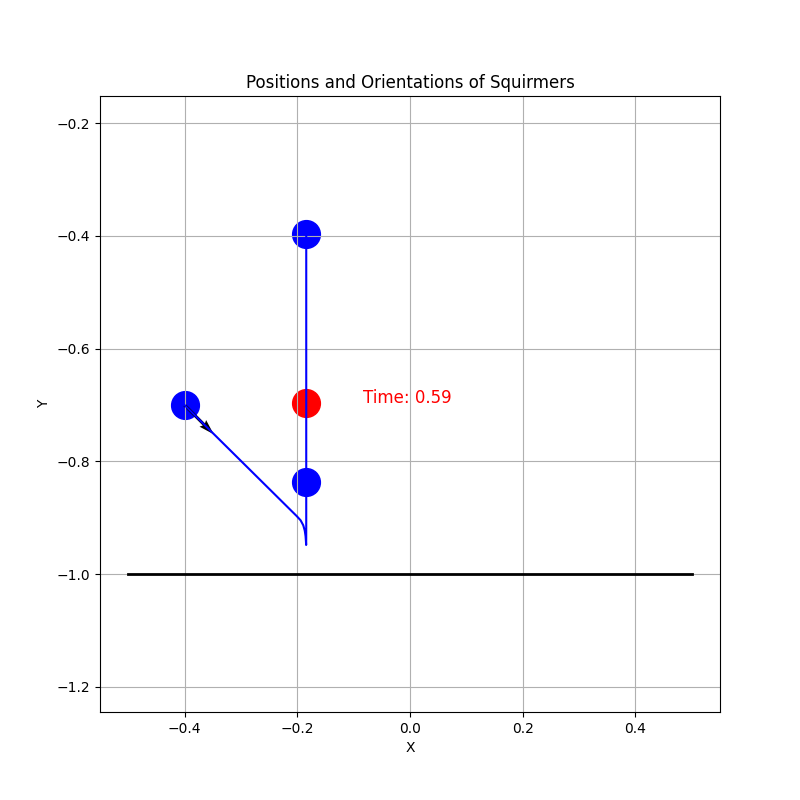
\includegraphics[width=1.1\textwidth]{graphs/simulations/border/betam3/mpi_4.png}
        \caption{\footnotesize $\beta = -3$}
    \end{minipage}
\end{figure}
\begin{figure}[H]
    \centering
    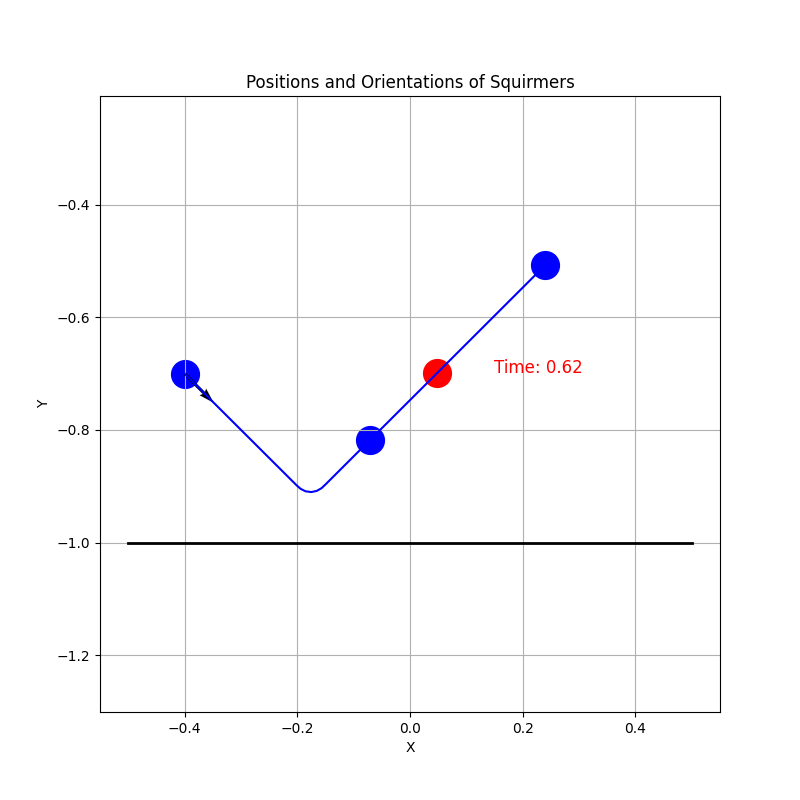
\includegraphics[width=0.55\textwidth]{graphs/simulations/border/beta0/mpi_4.png}
    \caption{\footnotesize $\beta = 0$}
    Simulation parameters: radius $a=0.05$, velocity $v_0=1$, simulation time $T=0.9$\\
        position and orientation of squirmer: $(x_1,y_1)=(-0.4,-0.7)$, $\theta=-\frac{\pi}{4}$
\end{figure}
Our results shows that for $\theta = -\frac{\pi}{4}$, as $\beta$ increases, the squirmer's orientation upon interaction becomes parallel to the border.
Conversely, as $\beta$ decreases, the squirmer's orientation upon interaction becomes tangential to the border.\\
One can note that the initial orientation has an impact on the orientation after interaction with the border as for $\theta = -\frac{\pi}{4}$ and 
$\beta = 1.5$, the squirmer reaches and exceeds the original height during the simulation time. In contrast, for $\theta = -\frac{\pi}{6}$ and 
$\beta = 1.5$, the squirmer does not reach the initial height.

\subsection{$E_0$ parameter}
The first thing done during the internship was to study the effect of the $E_0$ parameter on the alignment of the squirmers.\\
One can see the simulations done and their resulting graphs in the \texttt{graphs/Eo\_analysis} and \texttt{videos/Eo\_analysis} directories.\\
One also can type:
\begin{verbatim}
    python3 Code/run.py Eo_sim 2 filename
\end{verbatim}
and modify the \texttt{Code/run.py} file with the parameters one wants to test,
 then for each $E_0$ in \texttt{Code/run.py} and each $orient2$ and $betas$ in \texttt{sim\_Eo\_param} in \texttt{Code/simulation.py}, 
 a simulation is done and the resulting graphs or videos are stored in the \texttt{graphs} or \texttt{videos} 
 directory depending on one's choice.\\

\subsubsection{Evolution of orientation}
The evolution of the orientation of one squirmer is given by : 
$$
\frac{d \theta_i}{dt} = \sum \Gamma_{i(j)\rightarrow i} + \sum \Gamma_{j(i)\rightarrow i} +  \Gamma_{i}^W.
$$
$\Gamma_{ij\rightarrow k}$ is the torque exerted on the $k^\mathrm{th}$ particle by the flow associated to the $i^\mathrm{th}$ particle, but perturbed by the presence of the $j^\mathrm{th}$ particle.\\

\vspace{0.5cm}

The torques acting on the squirmer $i$ can be calculated explicitly by: \\
$$
\Gamma_{ij->i} = E_0(1 + \beta_i e_{ij})(-\ln\epsilon)\hat{e}_{ij}\times \hat{e}_i \cite{Lauga}
$$
and
$$
\Gamma_{ji->i} = \frac{1}{4}E_0(1 + \beta_j e_{ji})(-\ln\epsilon)\hat{e}_{ji}\times \hat{e}_j \cite{Lauga}
$$
with $\hat{e}_{ij} = \frac{(x_j - x_i)}{||x_j - x_i||}$, $e_{ij} = \hat{e}_i\cdot \hat{e}_{ij}$ and $E_0$ the parameter to test.\\ 
For squirmers having the same $\beta$ parameter we note the following relation:
$$
\Gamma_{ji->i} = \frac{1}{4}\Gamma_{ij->i}
$$
We want to study the effect of $E_0$ on the alignment of squirmers in an open environment so $\Gamma_{i}^W$, which is the torque 
exerted by a wall on the squirmer, is not used.

\subsubsection{Numerical Experiments}
The simulations are done with two squirmers placed at coordinates $(x_1, y_1) = (-a, 0)$ and $(x_2, y_2) = (\frac{2a}{1.5}, 0)$ with radius $a=0.05$, velocity $v_0=1$, viscosity $\mu = 1$, $\beta$ varying from $\beta_1 = 0$,
 $\beta_2 = -7.5$ and $\beta_3 = 7.5$, orientation $\theta_1 = \frac{\pi}{2}$ and $\theta_2$ varying between the major orientations of the unit circle.\\
 The value chosen for the $E_0$ parameter are chosen from the previous studies or to test the impact of larger values on the squirmers, such as:
 $$
 E_{0_{1}} = \frac{3}{10}\frac{v_0}{a}, E_{0_{2}} = \frac{8}{5}\mu\pi a^2 \cite{Brumley}, E_{0_{3}} = \frac{-3}{2}\frac{v_0}{a} \cite{Lauga},
 E_{0_{4}} = -E_{0_{1}}, E_{0_{5}} = -5$$
 $$
 E_{0_{6}} = \frac{5}{1000}, E_{0_{7}} = -2, E_{0_{8}} = -\frac{1}{2}, E_{0_{9}} = -E_{0_{8}}
 $$
The focus is for $\theta_2 = \pi$ and $\theta_2 = \frac{3\pi}{4}$ as the interactions are the biggest when the two squirmers are about to collide.
\begin{figure}[H]
    \centering
    \textbf{$\beta_1$ and $\theta_2 = \pi$}\par\medskip
    \begin{minipage}{0.49\textwidth}
        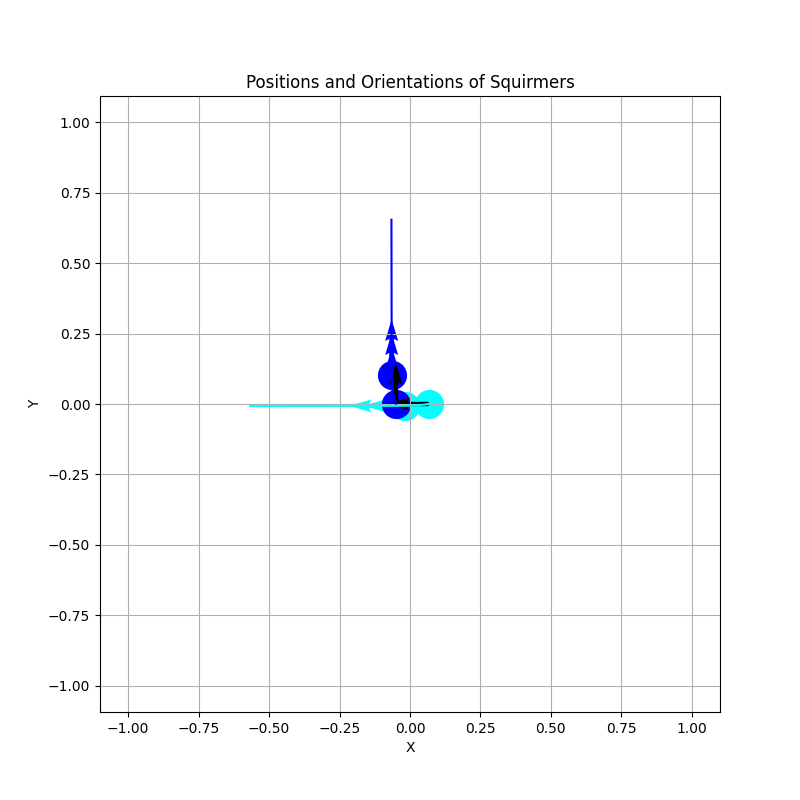
\includegraphics[width=1\textwidth]{graphs/Eo_analysis/beta0/pi_/pi_Eo_brumley.png}
        \caption{\footnotesize Simulation parameters: $a=0.05$, $v_0=1$, $\beta_1=0$, $\mu=1$ and $E_{0_{2}}=\frac{8}{5}\mu\pi a^2$}
    \end{minipage}\hfill
    \begin{minipage}{0.49\textwidth}
        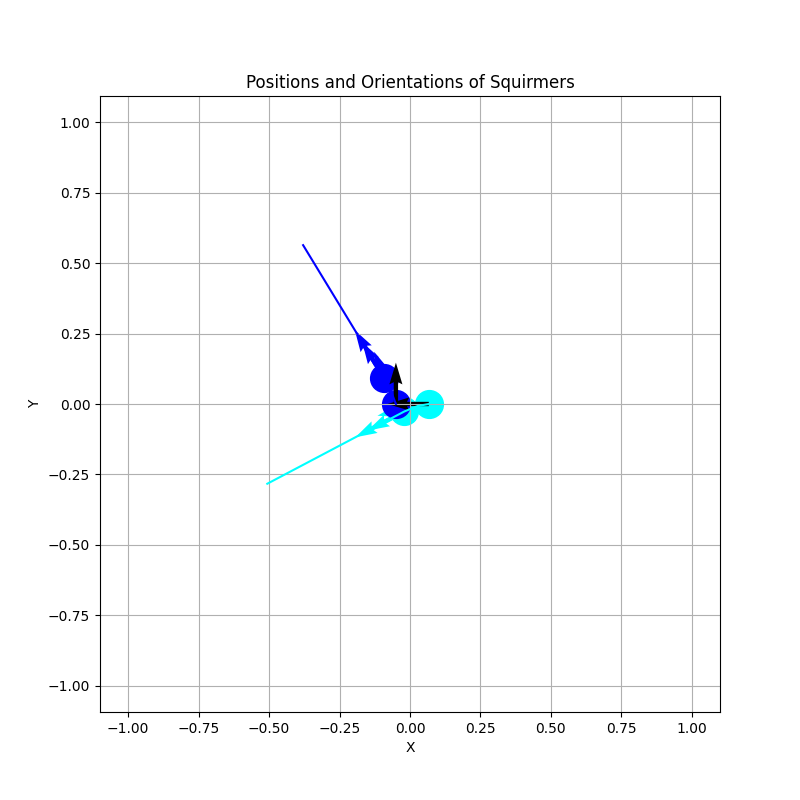
\includegraphics[width=1\textwidth]{graphs/Eo_analysis/beta0/pi_/pi_Eo_init.png}
        \caption{\footnotesize Simulation parameters: $a=0.05$, $v_0=1$, $\beta_1=0$, $\mu=1$ and $E_{0_{1}}=\frac{3}{10}\frac{v_0}{a}$}
    \end{minipage}
    \begin{minipage}{0.49\textwidth}
        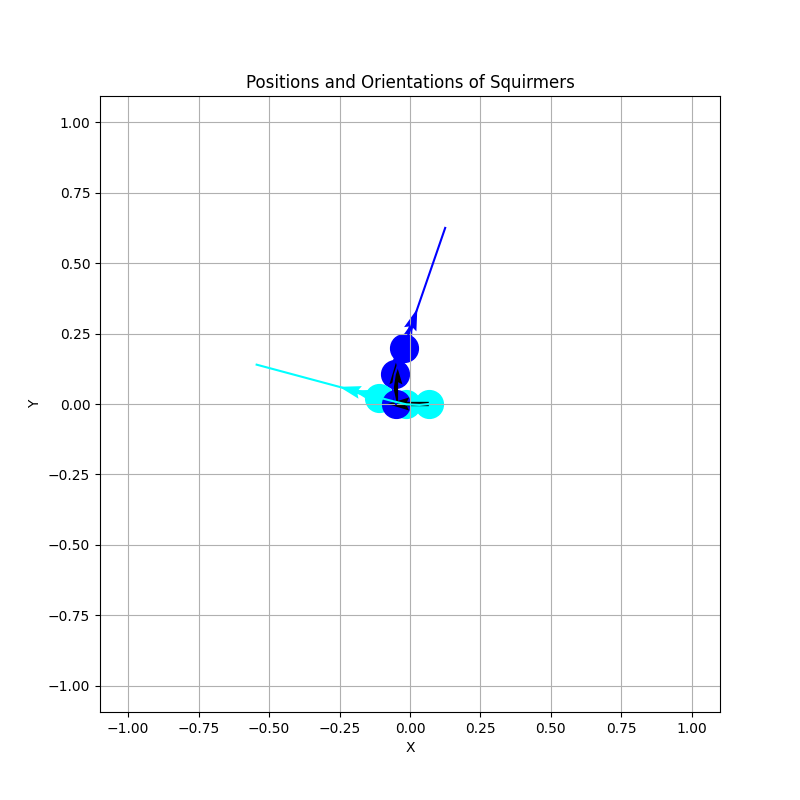
\includegraphics[width=1\textwidth]{graphs/Eo_analysis/beta0/pi_/pi_m2.png}
        \caption{\footnotesize Simulation parameters: $a=0.05$, $v_0=1$, $\beta_1=0$, $\mu=1$ and $E_{0_{7}}=-2$}
    \end{minipage}\hfill
    \begin{minipage}{0.49\textwidth}
        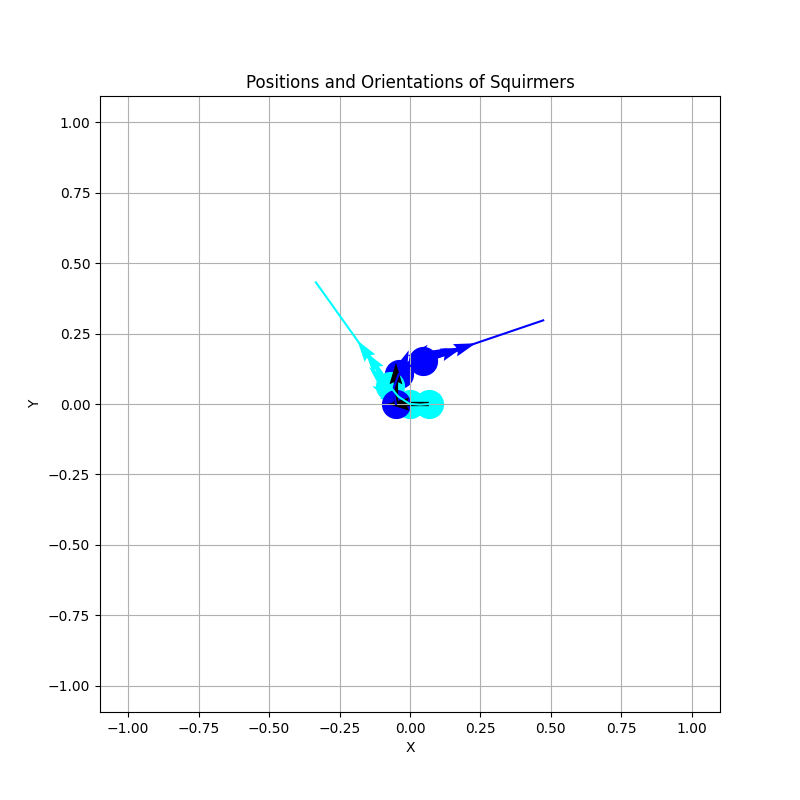
\includegraphics[width=1\textwidth]{graphs/Eo_analysis/beta0/pi_/pi_m5.png}
        \caption{\footnotesize Simulation parameters: $a=0.05$, $v_0=1$, $\beta_1=0$, $\mu=1$ and $E_{0_{5}}=-5$}
    \end{minipage}
    position and orientation of squirmer1: $(x1,y1)=(-a,0)$, $\theta_1=\frac{\pi}{2}$\\
    position and orientation of squirmer2: $(x2,y2)=(\frac{2a}{1.5},0)$, $\theta_2=\pi$\\
    The arrows shows when the orientations of the squirmers are affected and a circle is plotted every four time the orientation of a squirmer is affected
\end{figure}

\subsection{N squirmers}
The first step was to modify the code done during the initial project to simulate the behavior of $N$ squirmers.

\newpage

\nocite{*}
\bibliographystyle{plain}
\bibliography{bibliography/biblio}
\end{document}
